% !TEX program = xelatex
%\documentclass[10pt]{beamer}
\documentclass[hyperref={pdfpagemode=FullScreen},aspectratio=169,10pt]{beamer}
\usetheme[subsectionpage=progressbar]{metropolis}
\setbeamertemplate{section in toc}[sections numbered]
\setbeamertemplate{subsection in toc}[subsections numbered]
\metroset{progressbar=frametitle}
\metroset{numbering=none}
%W\usepackage[utf8]{inputenc}
\usepackage{ragged2e}
\usepackage{ulem}
\usepackage{caption}
\usepackage{amsmath}
\usepackage[mathrm=sym]{unicode-math}
 \setmathfont{Fira Math}
\usepackage{graphicx} 
\usepackage{outlines}
\usepackage{appendixnumberbeamer}
\usepackage{booktabs}
\usepackage[font=small,labelfont=bf]{caption}
\usepackage{hyperref}
\usepackage[scale=2]{ccicons}
\usepackage{caption}
\usepackage{subcaption}
\graphicspath{{../figures/}}
\usepackage{pgfplots}
\usepgfplotslibrary{dateplot}
\setsansfont[BoldFont={Fira Sans Bold}]{Fira Sans Book}
\usepackage{xspace}
\newcommand{\themename}{\textbf{\textsc{metropolis}}\xspace}
\theoremstyle{definition}
\metroset{block=fill}

\setbeamertemplate{footline}[text line]{%
  \parbox{\linewidth}{\vspace*{-8pt} \textbf{A. Tomašević} \hfill \textbf{07/08/21} \hfill \textbf{Networks 2021} \hfill \textbf{github.com/atomasevic/essnet}}}
\setbeamertemplate{navigation symbols}{}


\definecolor{Purple}{HTML}{911146}
\definecolor{Orange}{HTML}{CF4A30}
\setbeamercolor{alerted text}{fg=Orange}
\setbeamercolor{frametitle}{bg=Orange}
\renewcommand<>{\alert}[1]{\begin{alertenv}\bfseries#2#1\end{alertenv}}


\title{Detecting influential beliefs in large-scale surveys}
\date{July 2021}
\author{Aleksandar Tomašević}
\institute{University of Novi Sad}
%\titlegraphic{\hfill\includegraphics[height=1.9cm]{ff.pdf}}
\hbadness=99999
\begin{document}
\begin{frame}
  \titlepage
\end{frame}


% \begin{frame}
% \tableofcontents[hideallsubsections]
% \end{frame}


% \section{Research problem}

\begin{frame}{Overview}
  \Large
  1. \textbf{Motivation} - Belief systems in large surveys \\
  \vspace{1cm}
  2. \textbf{Analytical strategy} - Belief networks \\
  \vspace{1cm}
  3. \textbf{Results} - Influence of beliefs \\
  \vspace{1cm}
  4. \textbf{Future directions}

\end{frame}




\begin{frame}{Large-scale surveys}
  \large
  \begin{columns}[T]
    \begin{column}{.7\textwidth}

      \vspace{1cm}
      \begin{center}
        \textit{Cross-sectional \alert{Omnibus} Social Surveys Focusing on Social Behavior, Attitudes, and Values}
      \end{center}
      \pause
      \vspace{1cm}
      \begin{itemize}
        \item No single research goal
        \item Variety of topics and modules
      \end{itemize}
      % \alert{Belief system} construction
      % \alert{Influential beliefs?}

    \end{column}
    \hfill
    \begin{column}{.28\textwidth}
      
\includegraphics[width=2.5cm]{ess.png} \\
      
\includegraphics[width=2.5cm]{bsa.jpg} \\
      %
\includegraphics[width=2.9cm]{albus.jpeg} \\
      
\includegraphics[width=2.5cm]{gss.jpg}
    \end{column}
  \end{columns}
\end{frame}


\begin{frame}{Belief systems}

  \begin{columns}[T]

    \begin{column}{.51\textwidth}
      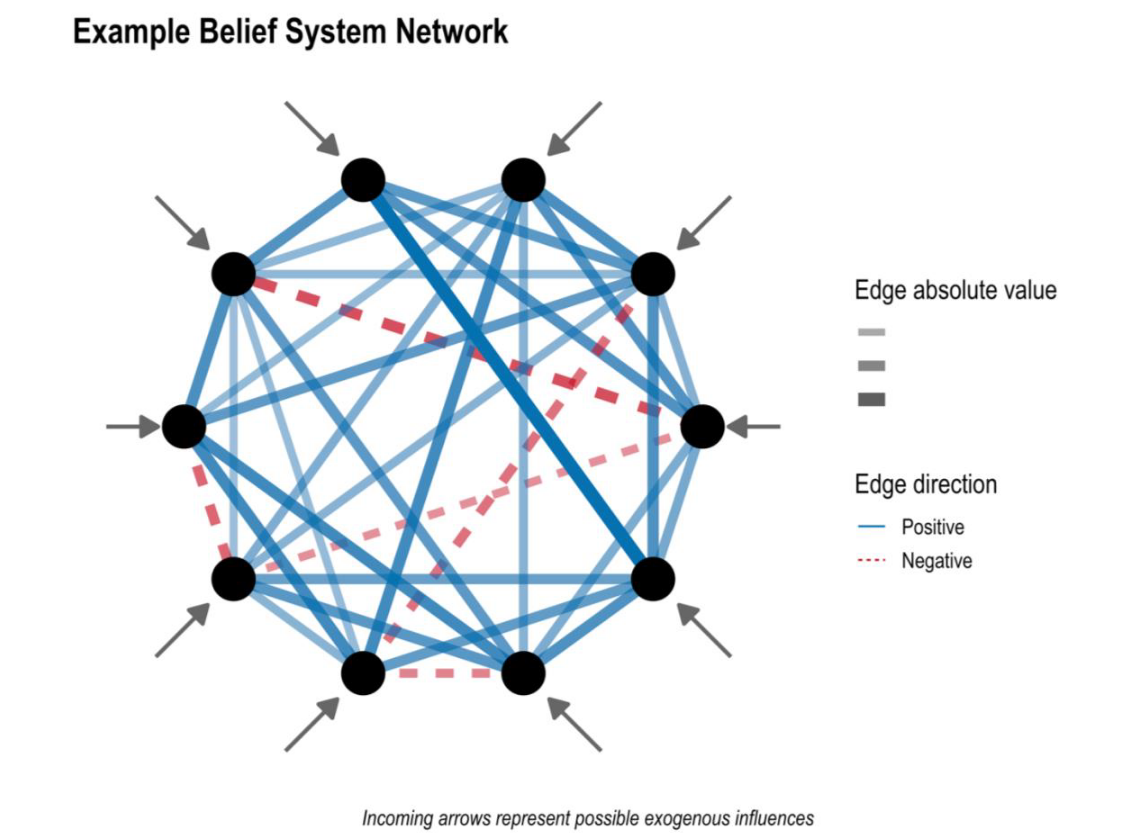
\includegraphics[width=6cm]{bs.png} \\
      \tiny
      \textit{Brandt, M. J., \& Sleegers, W. W. A. (2021). Evaluating Belief System Networks \\ as a Theory of Political Belief System Dynamics. \\ Personality and Social Psychology Review}
    \end{column}
    \hfill
    \begin{column}{.49\textwidth}

      \textbf{Beliefs} $=$  \alert{evaluations} or \alert{cognitive} aspects of attitudes
      \\
      \pause
      \vspace{0.5cm}

      \textbf{Belief System Networks} $=$ model of interrelationships between beliefs\\
      \pause
      \vspace{0.5cm}
      \textbf{Connectionist framework} \\ \pause \textbf{Network Flow}
    \end{column}
  \end{columns}

\end{frame}

\begin{frame}{Motivating example - European Social Survey}
  \Large
  \begin{columns}[T]
    \begin{column}{.55\textwidth}


      \pause
      \vspace{1cm}
      \begin{itemize}
        \item Round 9, 2018/2019
        \item 30 European countries
        \item \alert{Attitude towards national government}
      \end{itemize}

      % \alert{Belief system} construction
      % \alert{Influential beliefs?}

    \end{column}
    \hfill
    \begin{column}{.43\textwidth}
      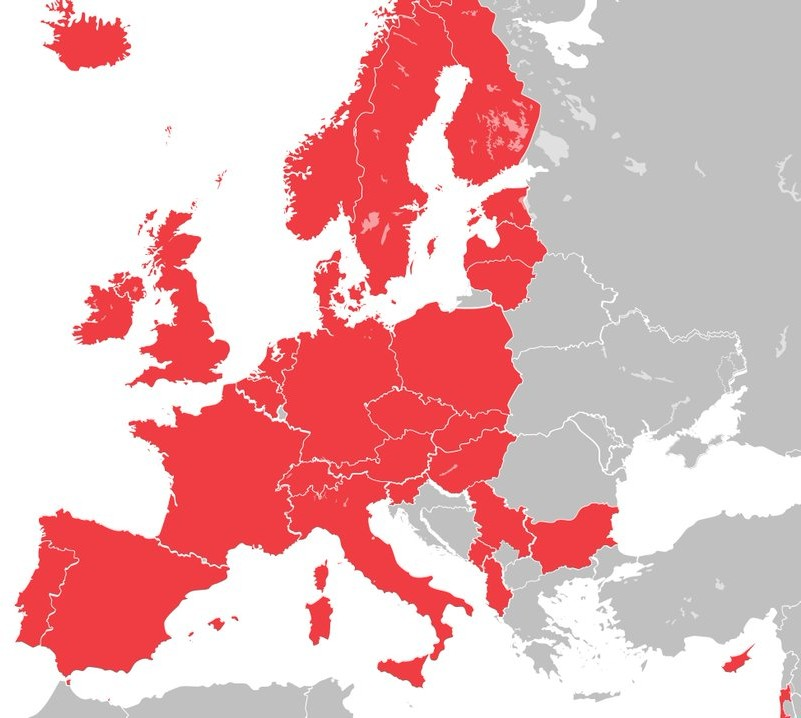
\includegraphics[width=4cm]{ess-map.jpg}
    \end{column}
  \end{columns}
  \vspace{2cm}
\end{frame}

\begin{frame}{Motivating example}
  \begin{columns}[T] % align columns
    \begin{column}{.48\textwidth}

      \begin{block}{Govermental Performance}
        Satisfaction with \alert{Economy} \\
        Satisfaction with \alert{Democracy} \\
        State of \alert{Healthcare}  \\
        State of \alert{Education}
      \end{block}

      \vspace{0.5cm}

      \begin{block}{Political Trust}
        \alert{Parliament} \\
        \alert{Legal system} \\
        \alert{Police}  \\
        \alert{Politicians}  \\
        \alert{Political parties}
      \end{block}

    \end{column}%
    \hfill%
    \begin{column}{.48\textwidth}
      \begin{block}{Representation \& Fairness}
        Systems allows people to have \alert{a say} \\
        Systems allows people to have \alert{influence}  \\
        Gov. decisions are \alert{transparent}   \\
        Gov. takes into account \alert{interests of all}  \\
        System gives a \alert{fair chance} to all
      \end{block}
    \end{column}%
  \end{columns}
\end{frame}
% \section{Belief network analysis}

\begin{frame}{Analytical strategy}

  \textbf{Unique Variable Analysis} (Christensen, Garrido \& Golino, 2020) \\
  \pause
  \vspace{0.2cm}
  \hspace{0.5cm} Weighted topological overlap (wTO, Zhang \& Horvath, 2005) \\
  \hspace{0.5cm} on partial correlation matrix \\
  \vspace{0.2cm}
  \textbf{Estimate Gaussian Graphical Model} \\
  \vspace{0.2cm} \hspace{0.5cm} graphical LASSO regularization, extended BIC for model selection \\
  \pause \vspace{0.2cm}
  \textbf{Split the sample \& test network differences}.\\
  \vspace{0.2cm}
  \textbf{Integrated Value of Influence} (IVI) \\(Salvaty, Ramialson \& Currie, 2020)
\end{frame}

\begin{frame}{UVA - Redundancy analysis}
  \begin{columns}[T] % align columns
    \begin{column}{.48\textwidth}

      \begin{block}{Govermental Performance}
        Satisfaction with \alert{Economy} \\
        Satisfaction with \alert{Democracy} \\
        State of \alert{Healthcare}  \\
        State of \alert{Education}
      \end{block}

      \vspace{0.5cm}

      \begin{block}{Political Trust}
        \alert{Parliament} \\
        \sout{\alert{Legal system}} \\
        \sout{\alert{Police}}  \\
        \alert{Politicians}  \\
        \sout{\alert{Political parties}}
      \end{block}

    \end{column}%
    \hfill%
    \begin{column}{.48\textwidth}
      \begin{block}{Representation \& Fairness}
        Systems allows people to have \alert{a say} \\
        \sout{Systems allows people to have \alert{influence}}  \\
        \sout{Gov. decisions are \alert{transparent}}   \\
        Gov. takes into account \alert{interests of all}  \\
        \sout{System gives a \alert{fair chance} to all}
      \end{block}
    \end{column}%
  \end{columns}
\end{frame}

{\setbeamercolor{background canvas}{bg=white} \begin{frame}
  \begin{flushleft}
    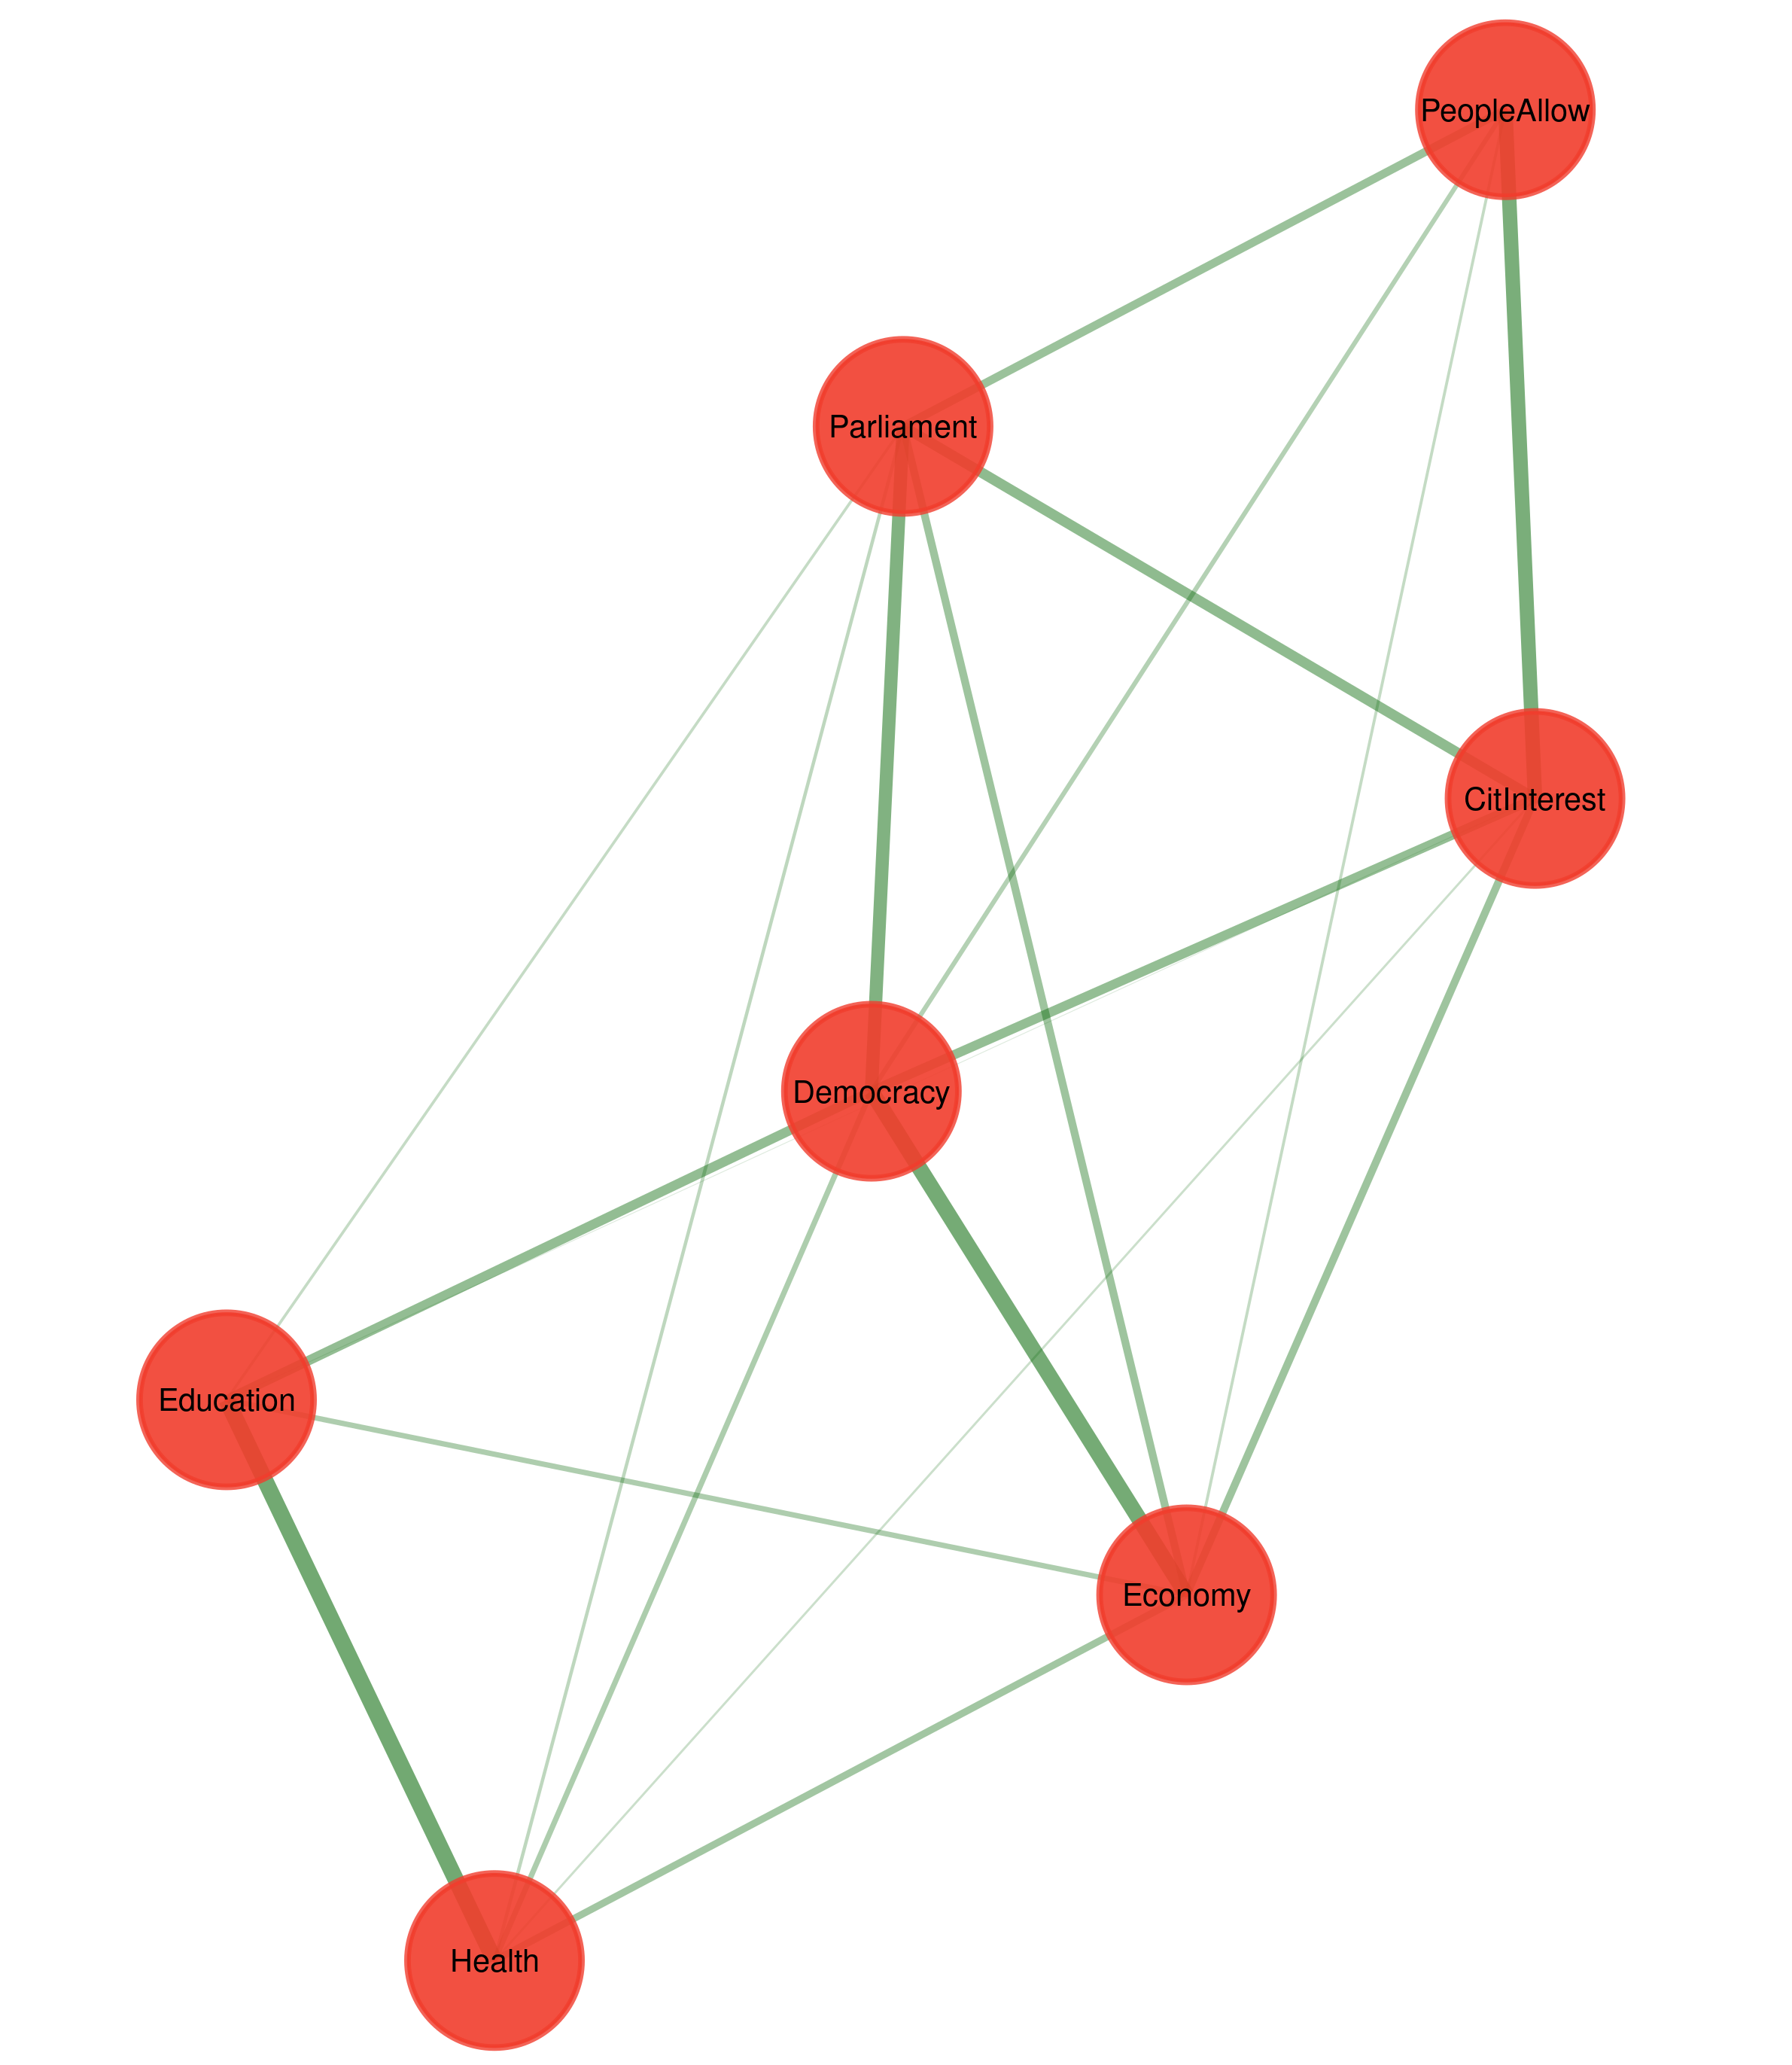
\includegraphics[width=0.47\paperwidth]{01-ega-full.png}
  \end{flushleft}
\end{frame}}

{\setbeamercolor{background canvas}{bg=white} \begin{frame}{\hspace{0.5cm}Electoral autocracies \hspace{0.5cm} VS \hspace{0.5cm} Liberal Democracies}
  \begin{figure}
    \begin{flushleft}
      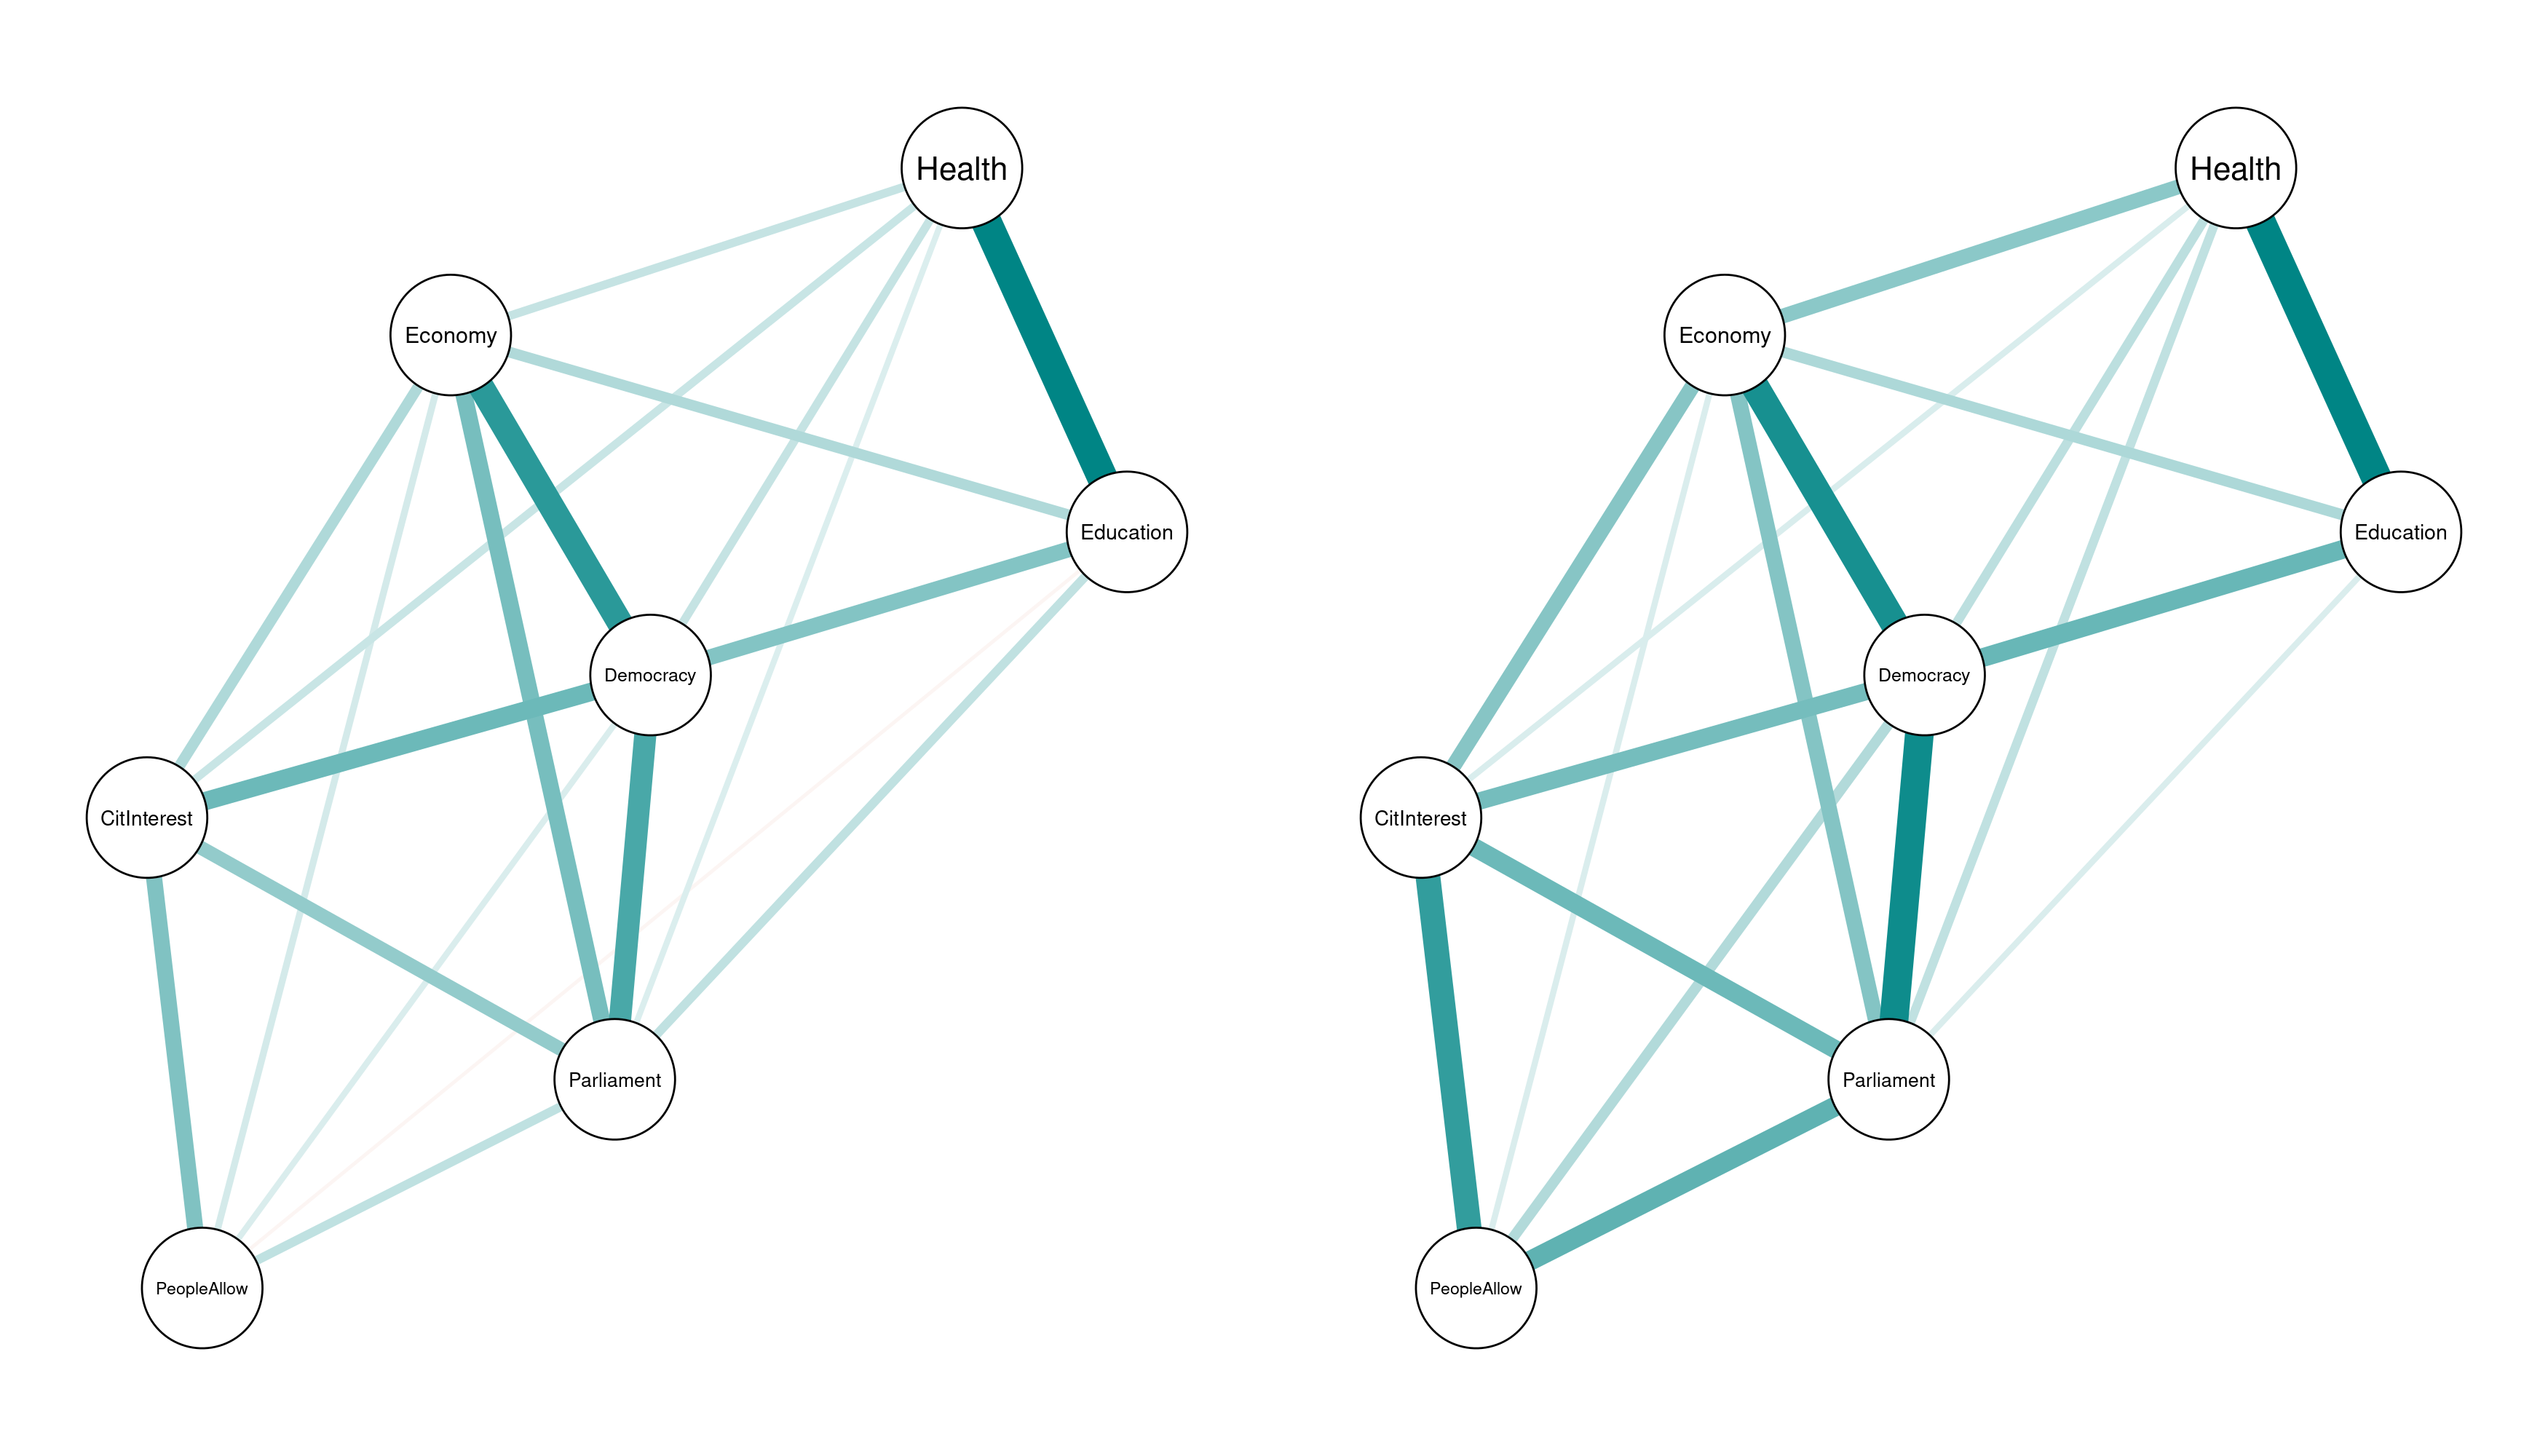
\includegraphics[width=0.75\paperwidth]{99-tree-ea-vs-ld.png}
    \end{flushleft}
  \end{figure}
\end{frame}}

\begin{frame}{IVI (Salvaty, Ramialson \& Currie, 2020)}
  \Large

  $$
    \mathrm{IVI}_i = (\mathrm{Hub}_i)(\mathrm{Spread}_i)
  $$
  % $$
  % \mathrm{IVI}_{i}=\left(\text { Hubness }_{\text {score }_{i}}\right)\left(\text { Spreading }_{\text {score }_{i}}\right)
  % $$
  \pause
  $$
    \mathrm{Hub}_i=\mathrm{DC}_{i}^{\prime}+\mathrm{LH}_{\mathrm {index }_{i}}^{\prime}
  $$

  $$
    \mathrm{Spread}_i =\left(\mathrm{NC}_{i}^{\prime}+\mathrm{CR}_{i}^{\prime}\right)\left(\mathrm{BC}_{i}^{\prime}+\mathrm{Cl}_{i}^{\prime}\right)
  $$

  \pause

\end{frame}







{\setbeamercolor{background canvas}{bg=white} \begin{frame}
  \begin{figure}
    \begin{flushleft}
      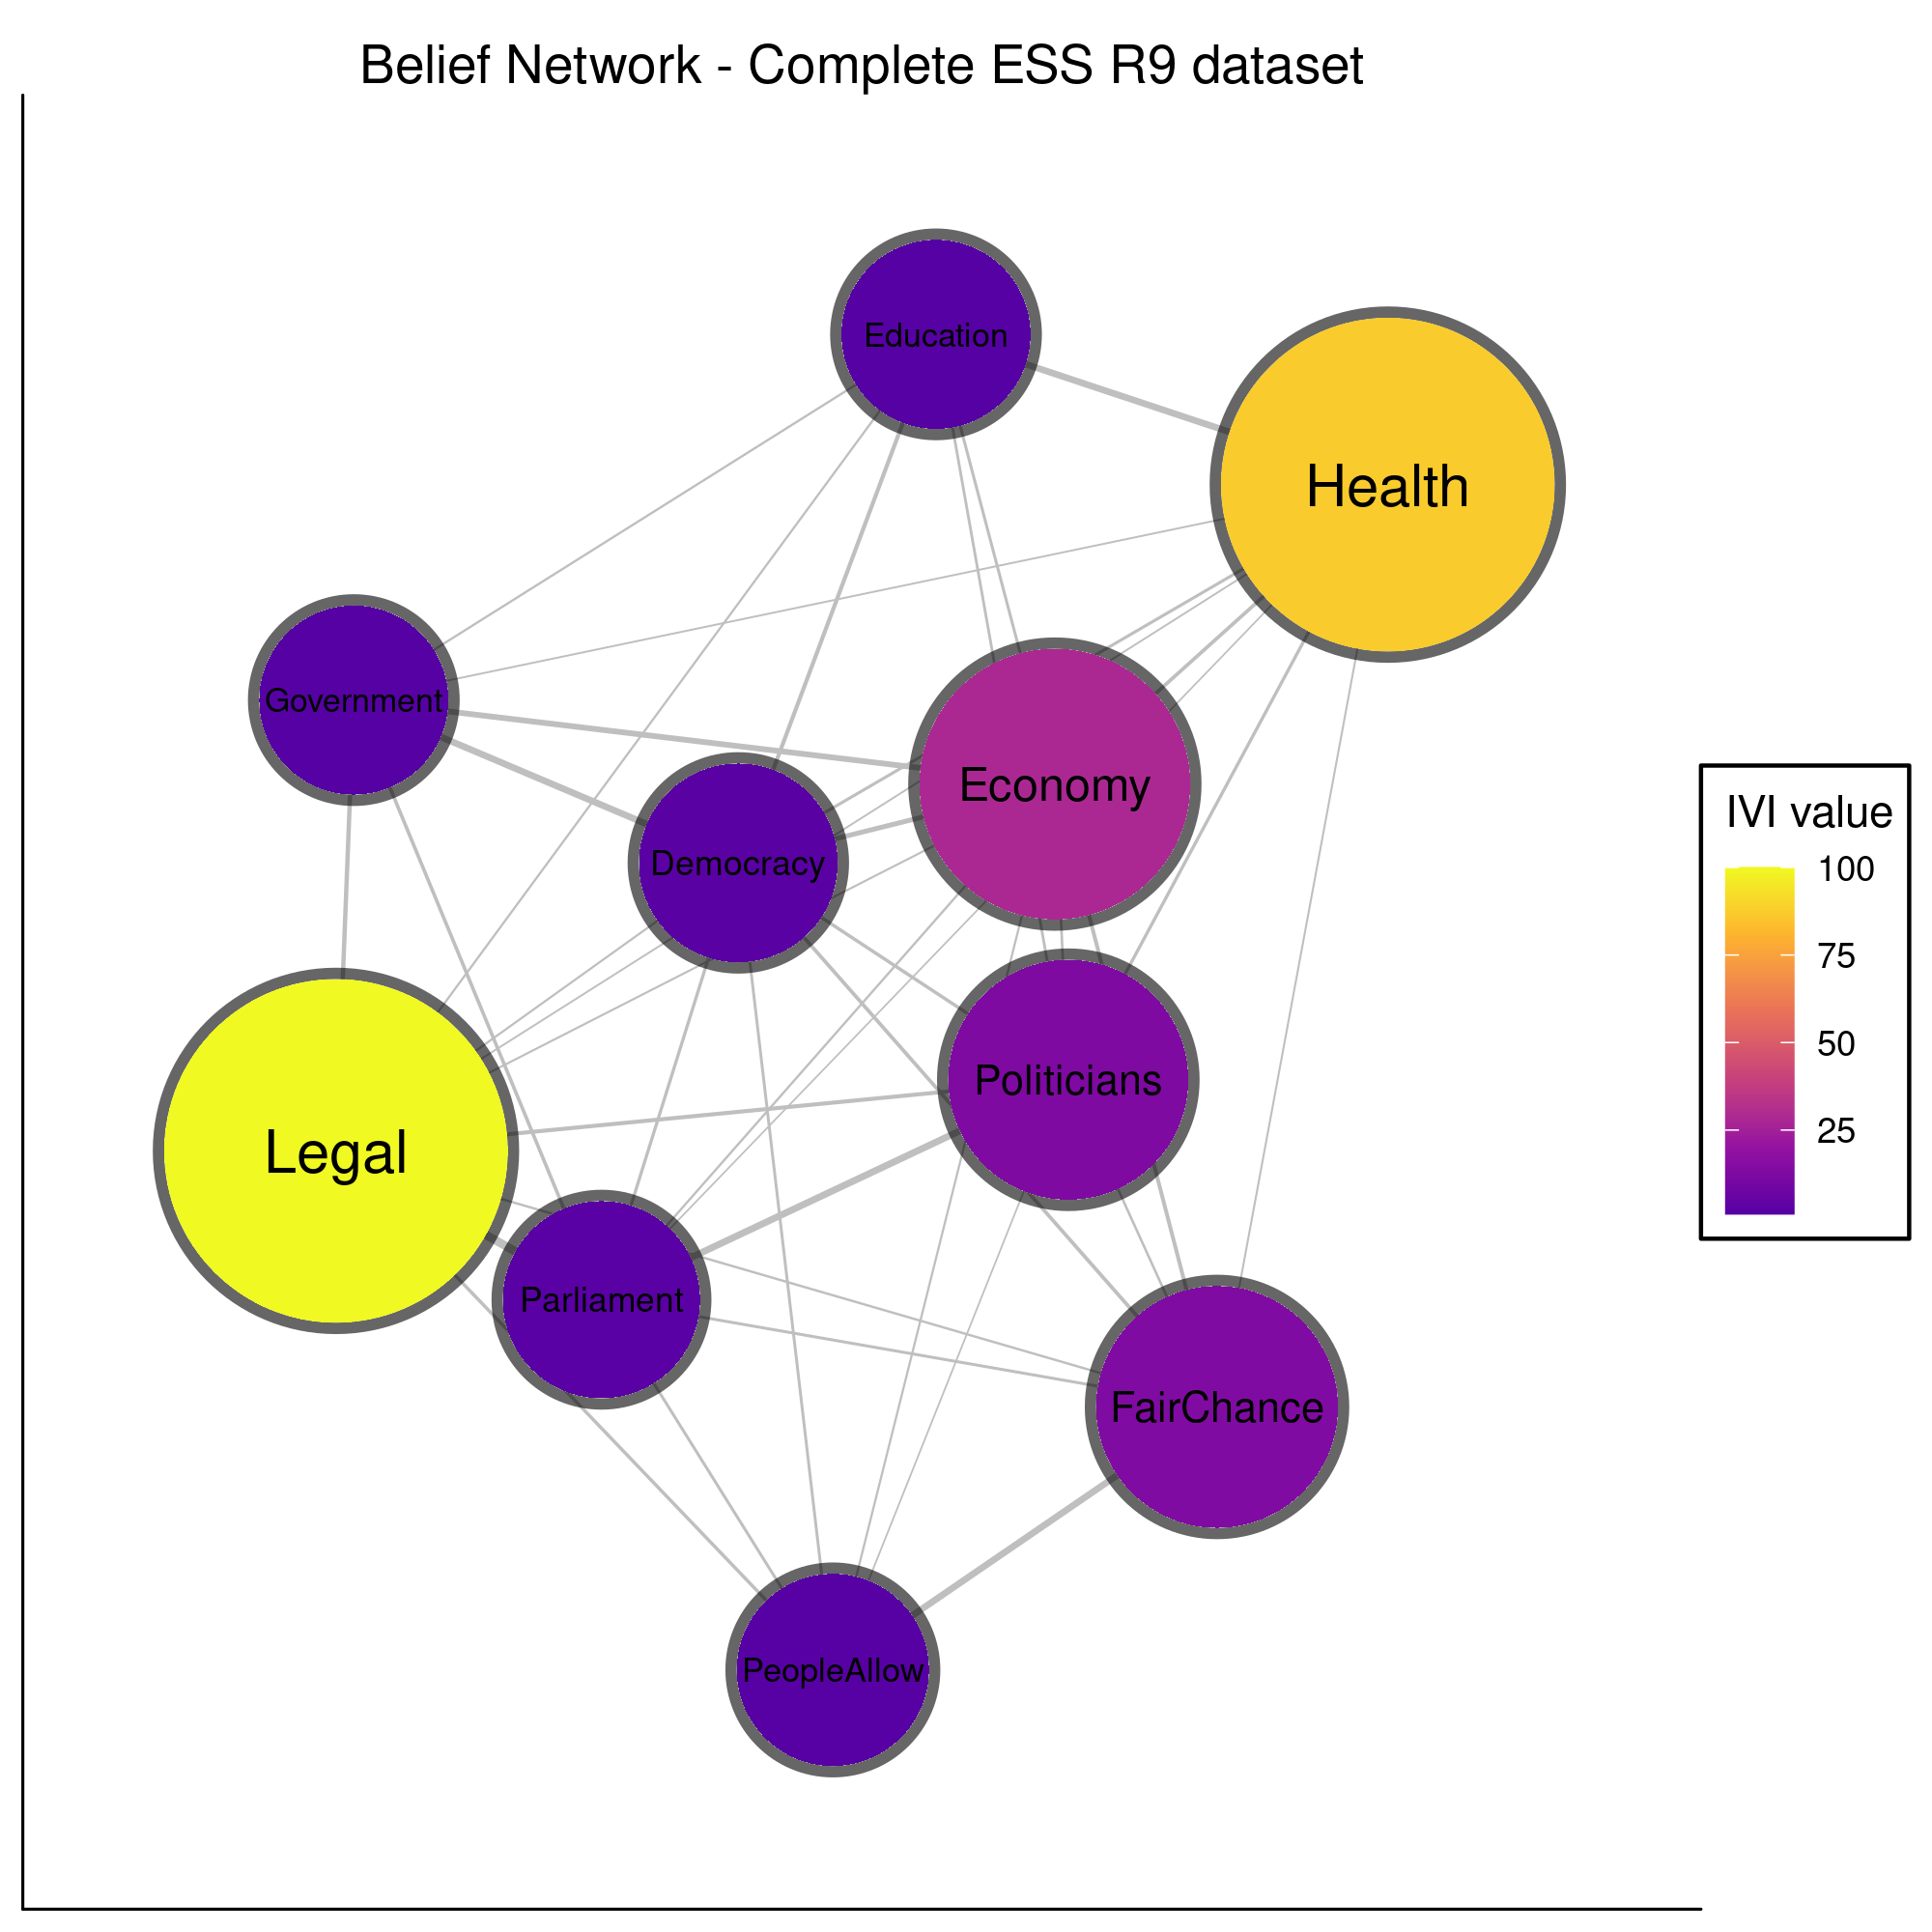
\includegraphics[width=0.58\paperwidth]{02-ivi-full.png}
    \end{flushleft}

  \end{figure}
\end{frame}}

{\setbeamercolor{background canvas}{bg=white} \begin{frame}
  \begin{figure}
    \begin{flushleft}
      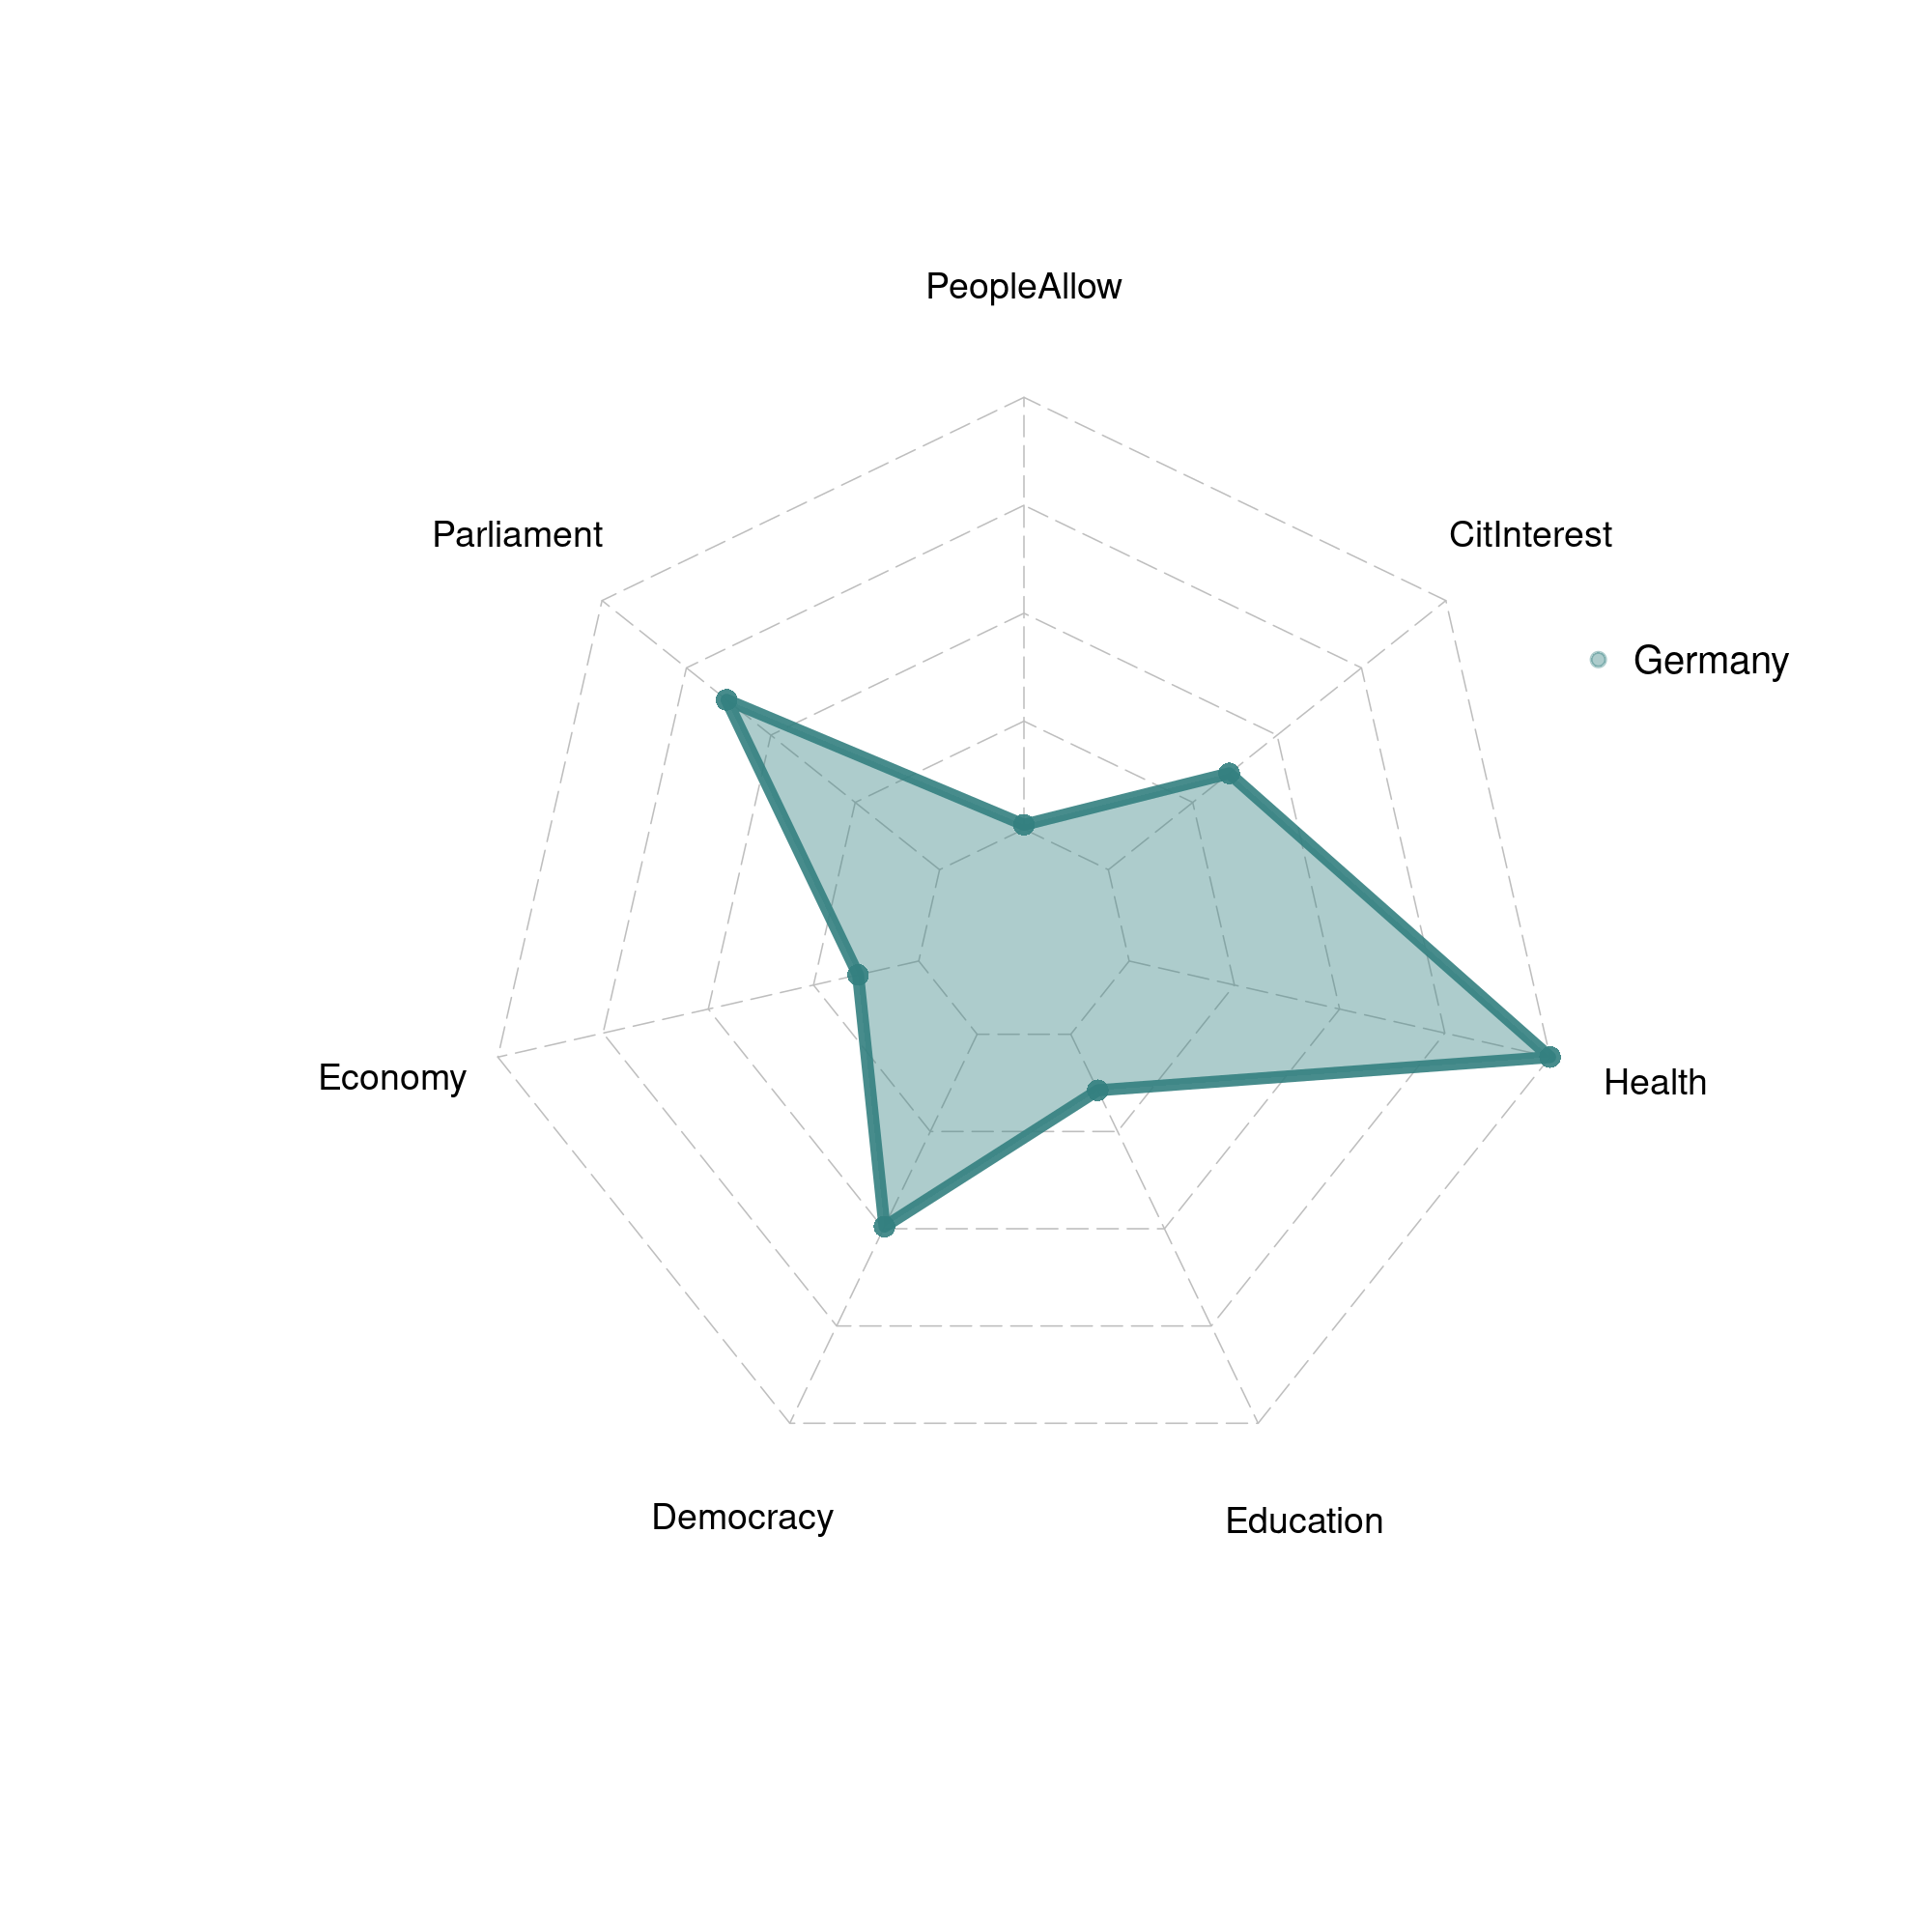
\includegraphics[width=0.65\paperwidth]{03-radar-ger.png}
    \end{flushleft}

  \end{figure}
\end{frame}}

{\setbeamercolor{background canvas}{bg=white} \begin{frame}
  \begin{figure}
    \begin{flushleft}
      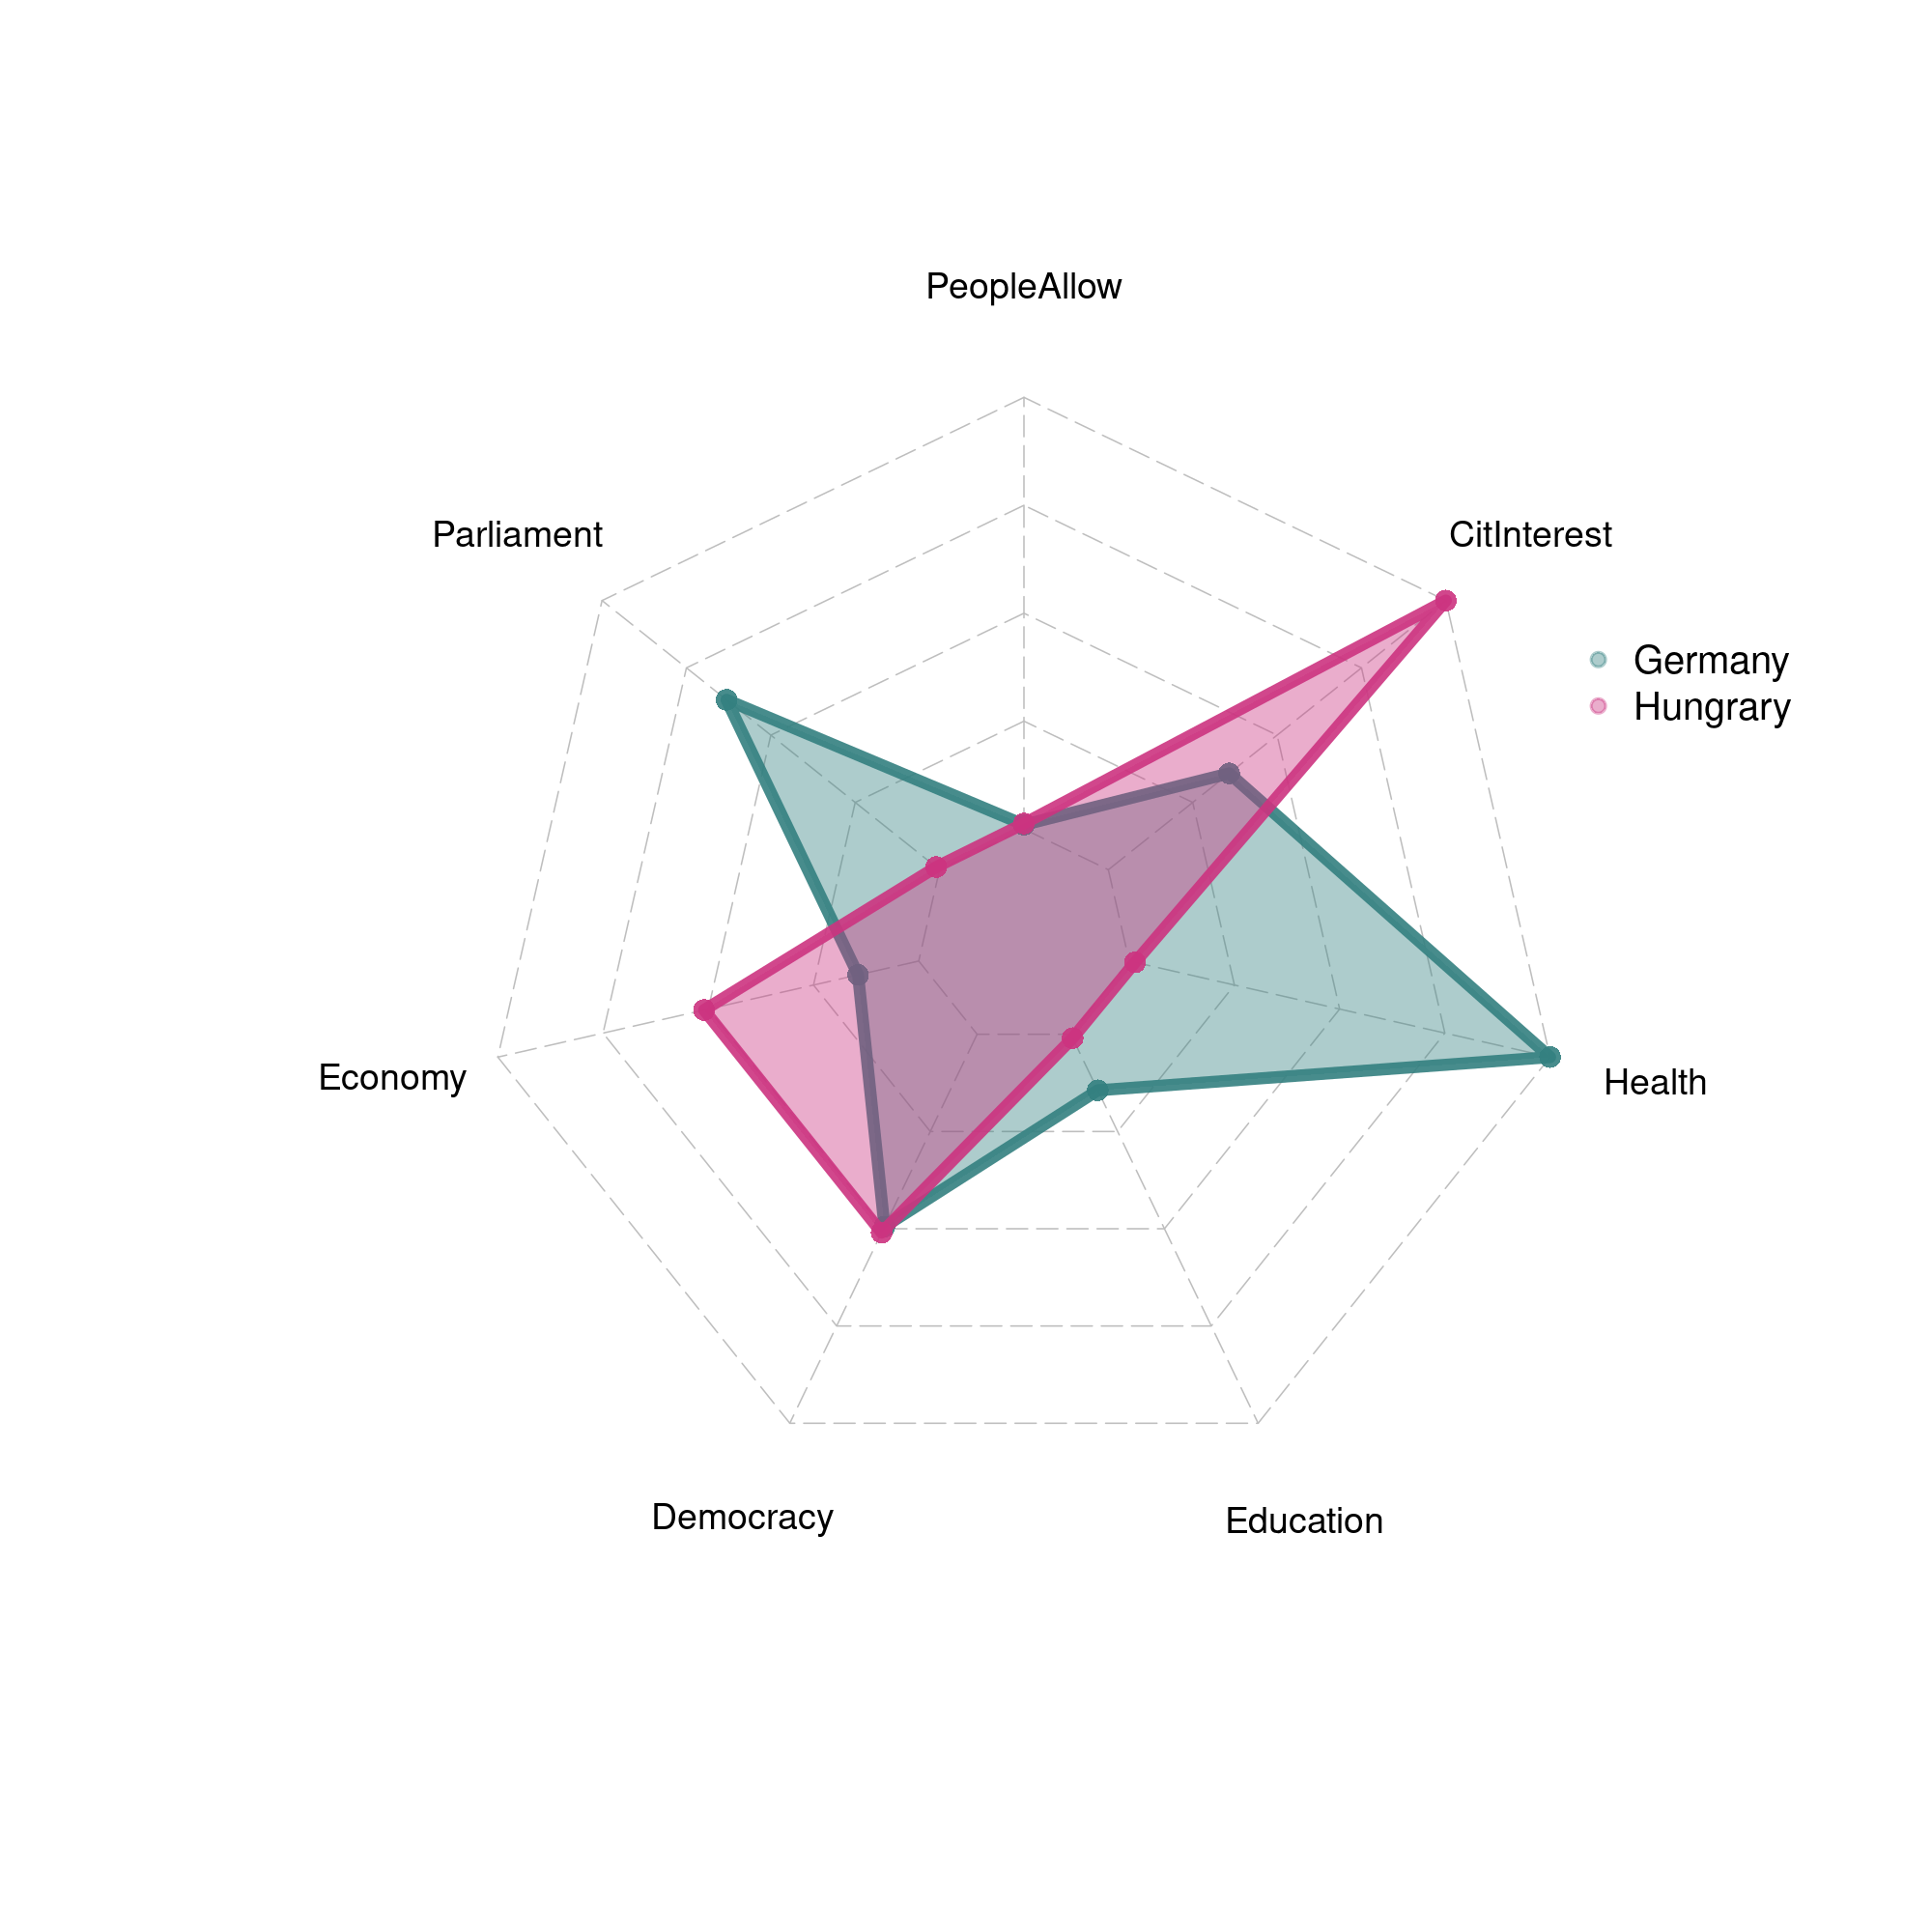
\includegraphics[width=0.65\paperwidth]{03-radar-ger-hu.png}
    \end{flushleft}
  \end{figure}
\end{frame}}

\setbeamercolor{background canvas}{bg=white}

\begin{frame}
  \begin{figure}
    \begin{flushleft}
      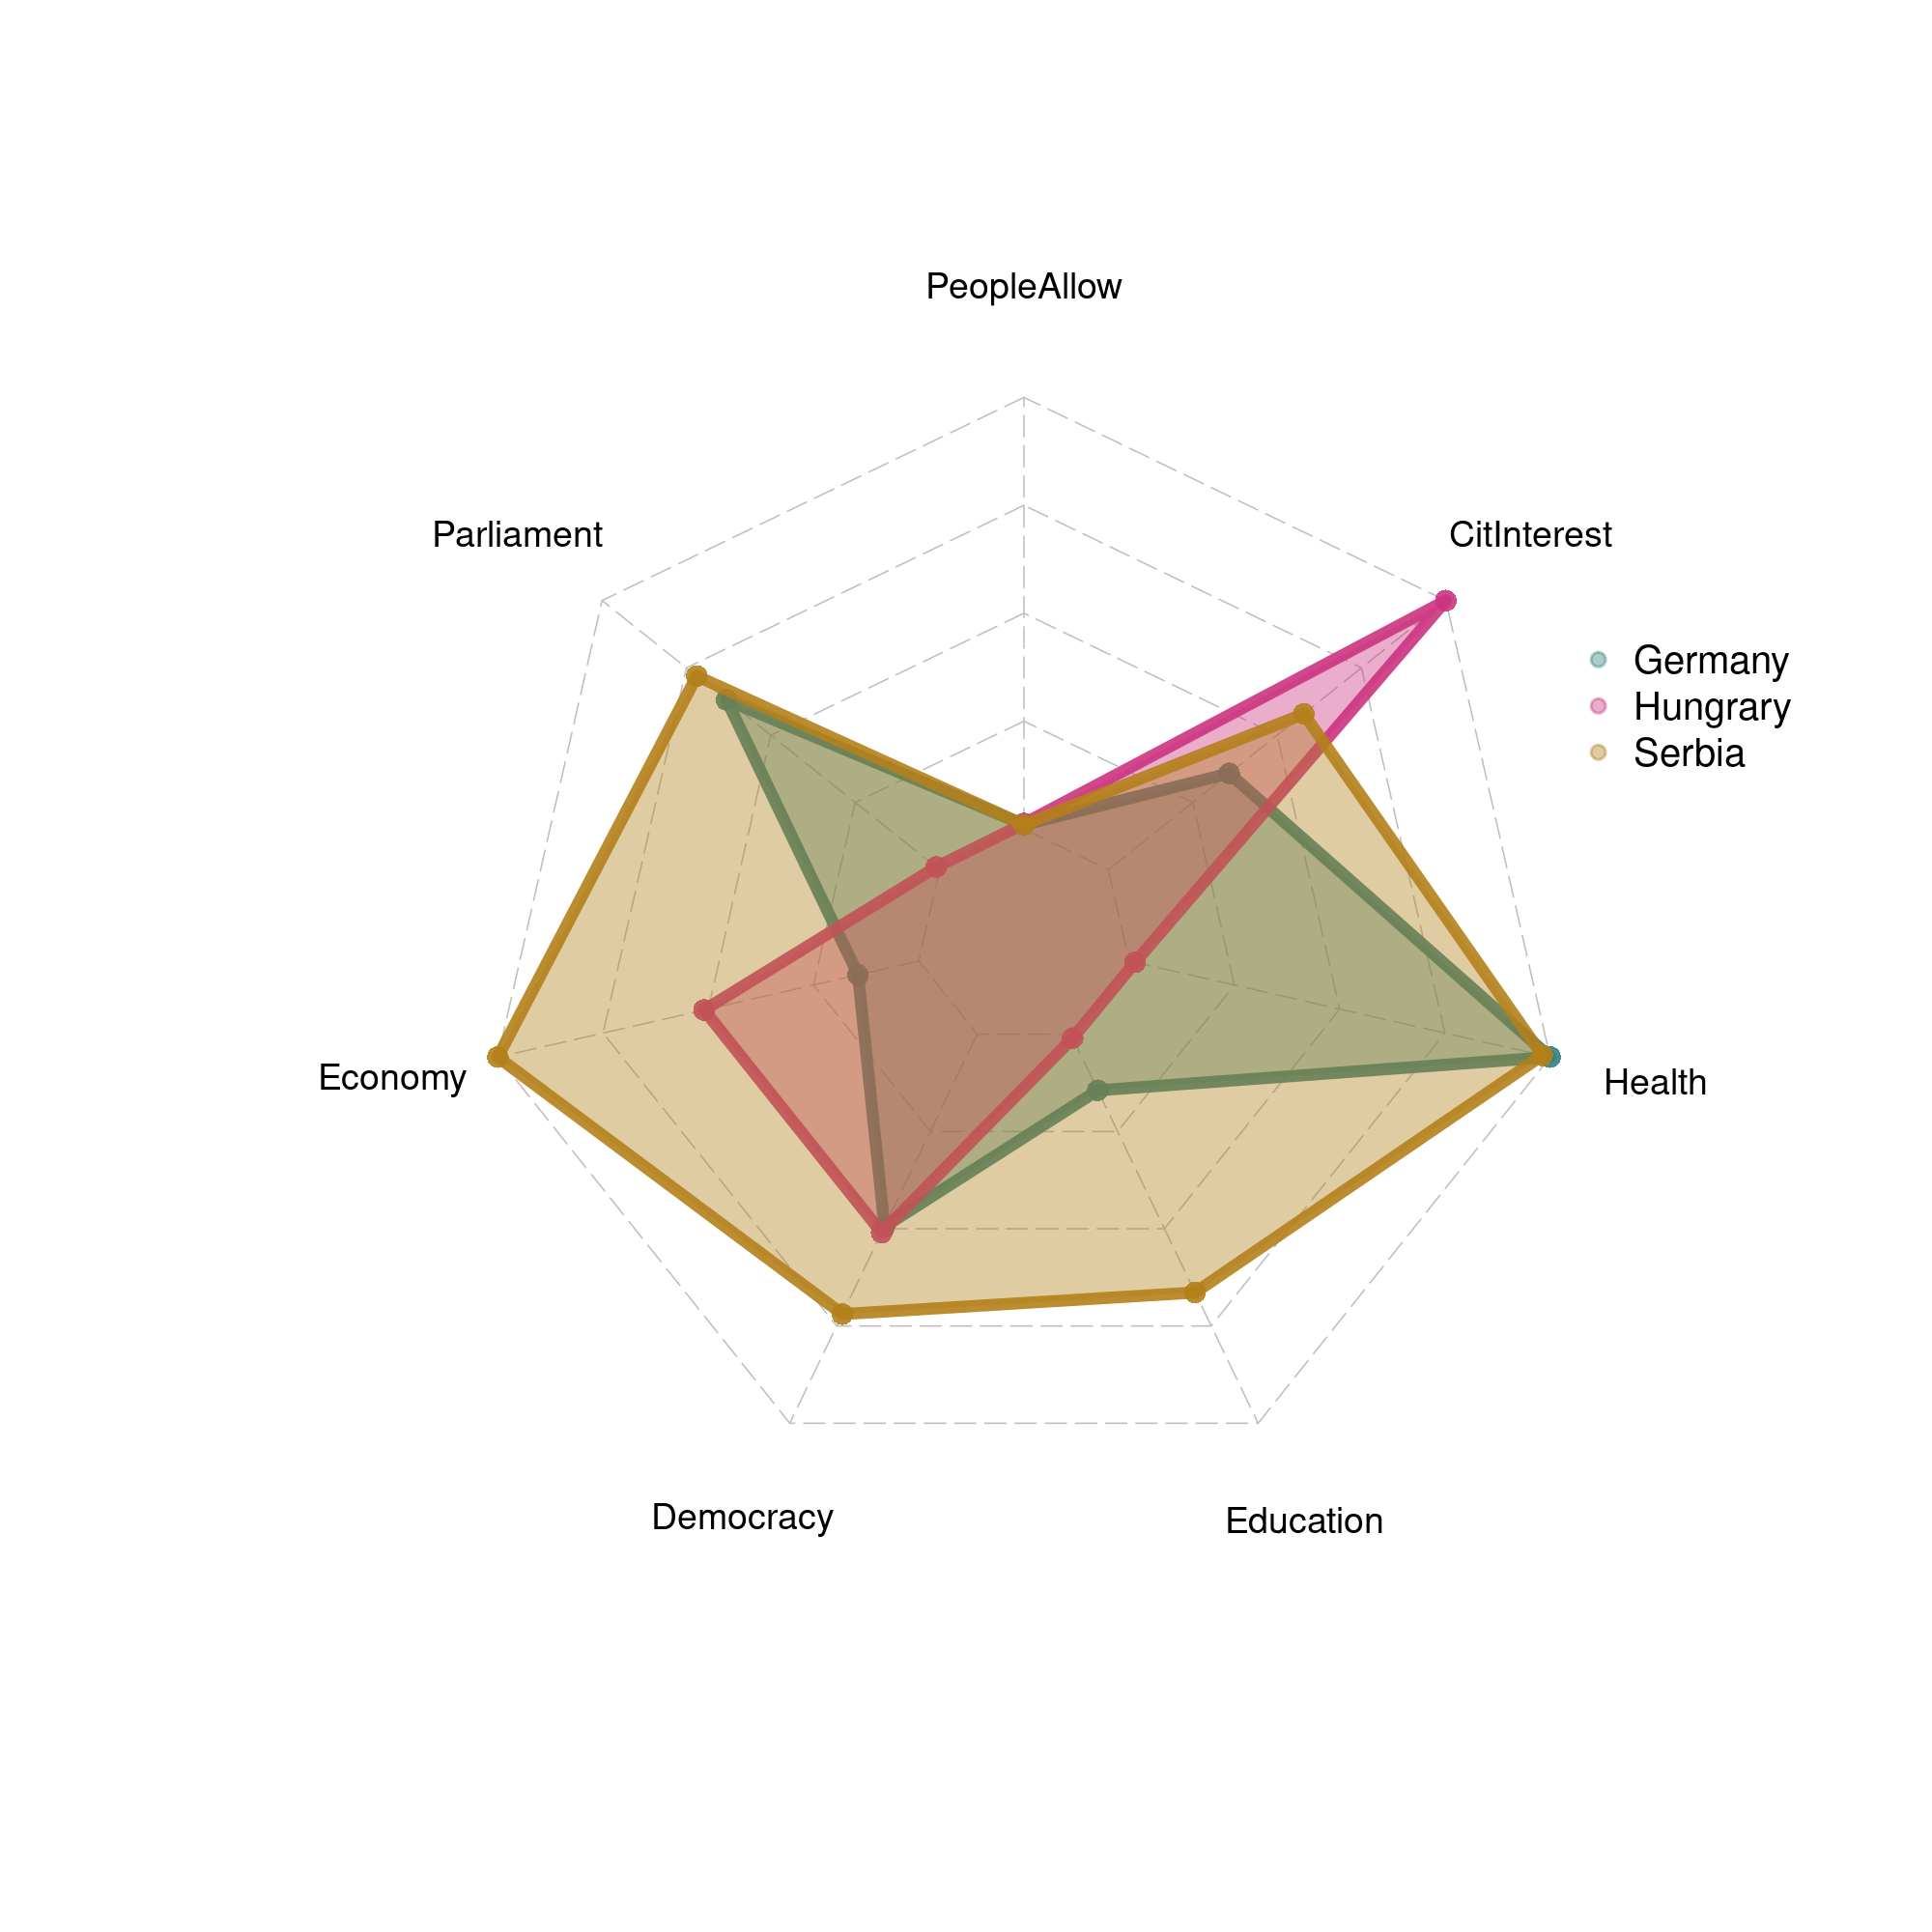
\includegraphics[width=0.65\paperwidth]{03-radar-hu-rs.png}
    \end{flushleft}
  \end{figure}
\end{frame}

\setbeamercolor{background canvas}{bg=white}
\begin{frame}{GDP per capita vs Economy IVI}
  \begin{figure}
    \begin{flushleft}

      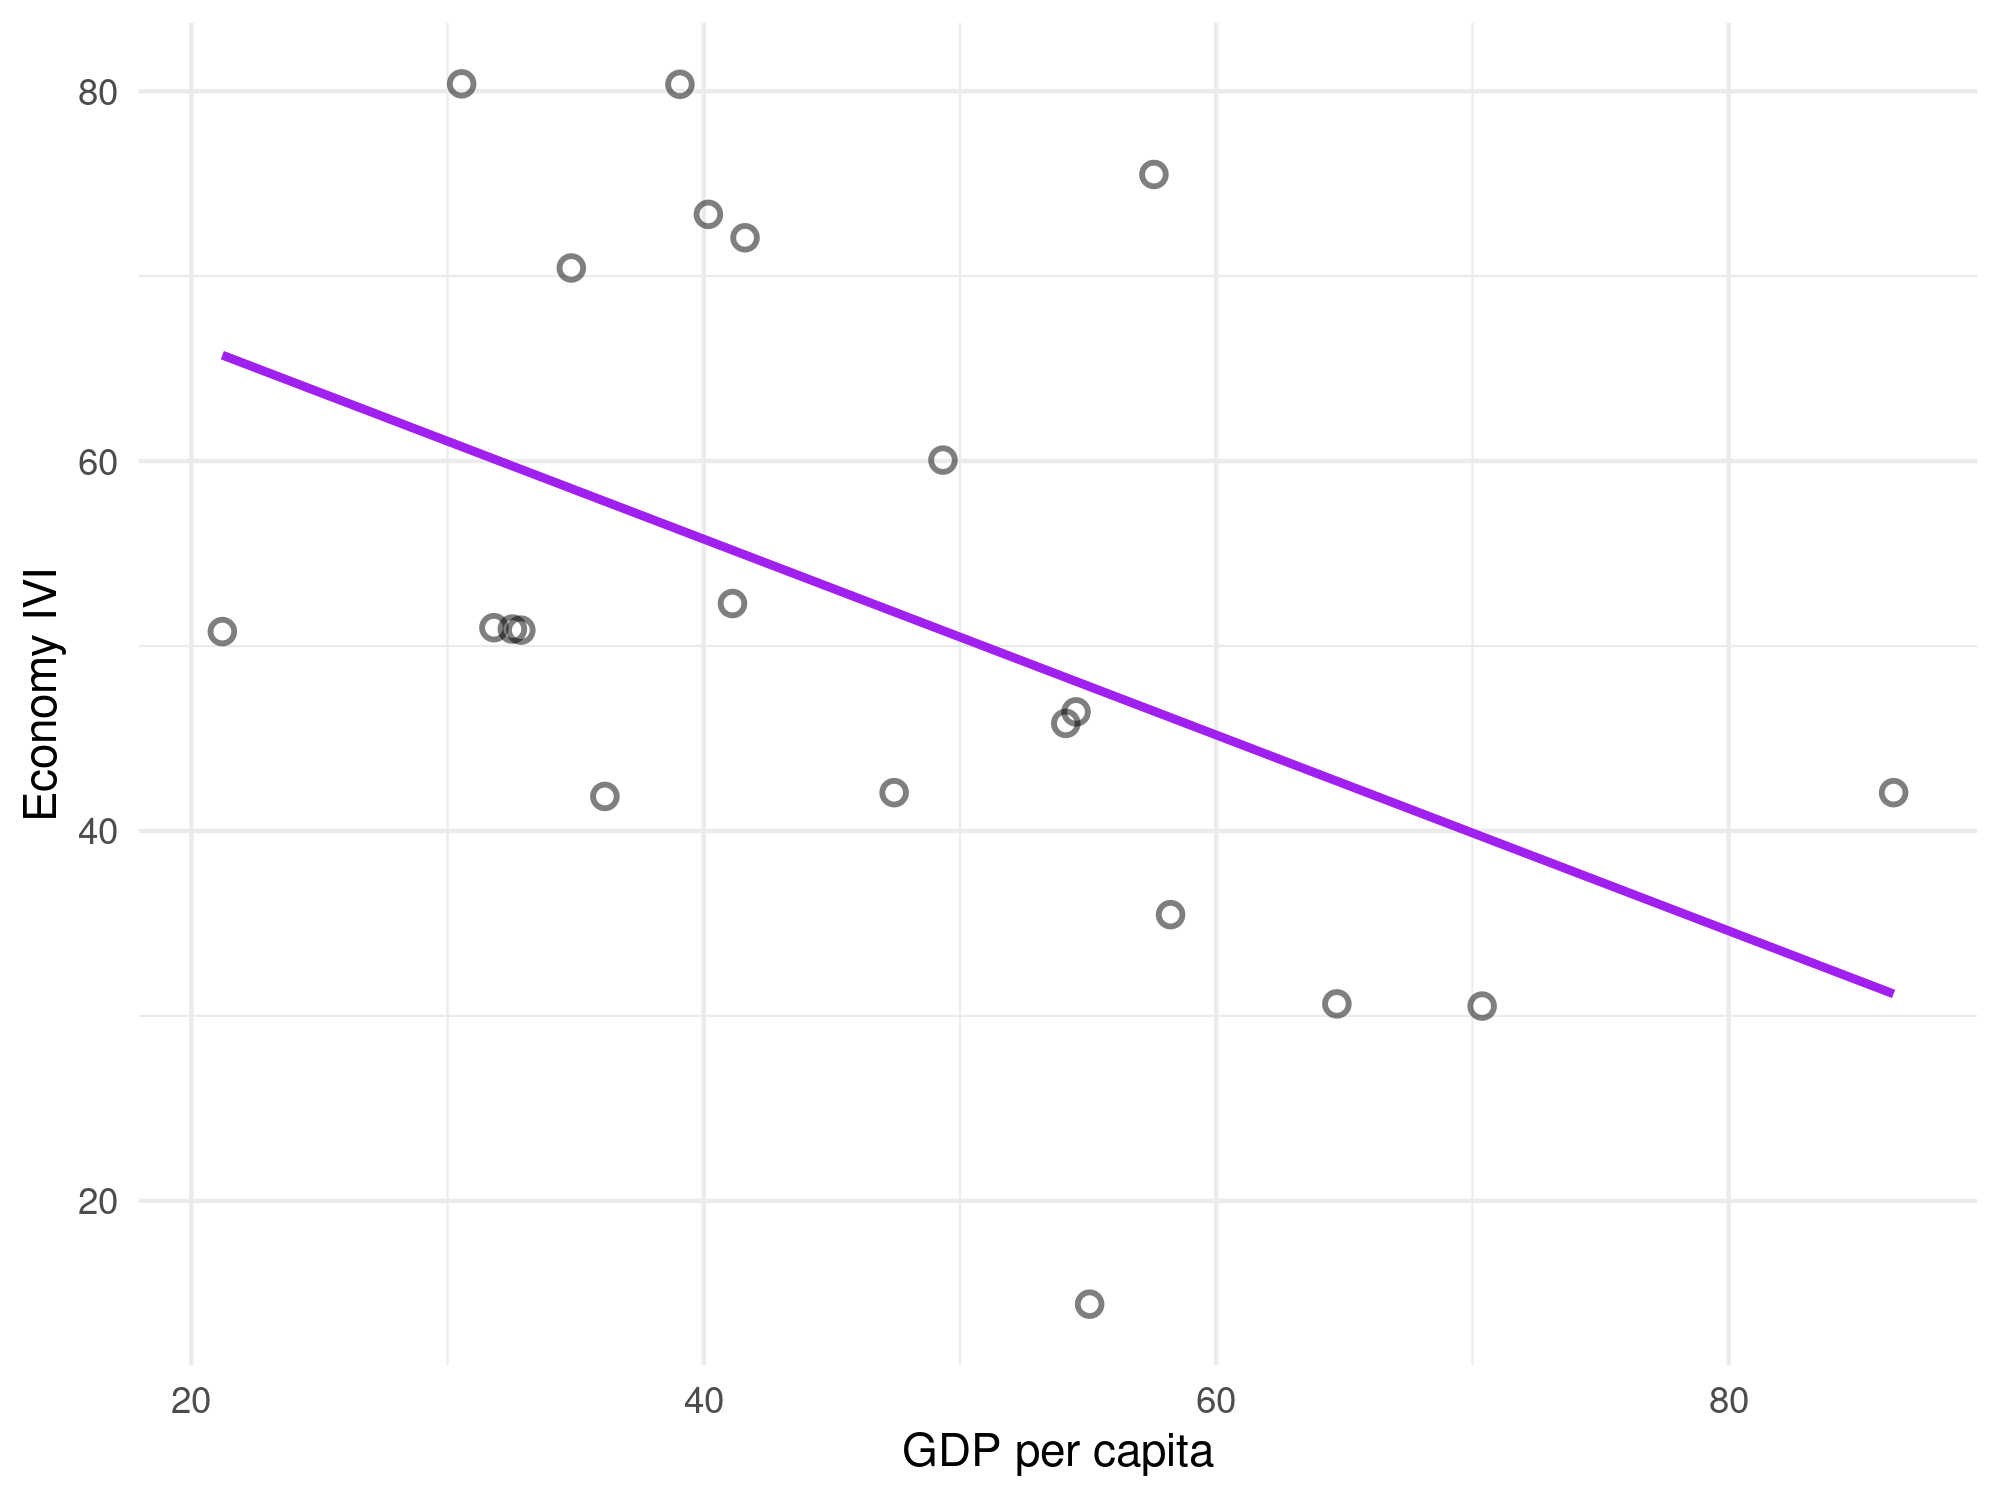
\includegraphics[width=0.5\paperwidth]{05-scatter-eco.png}
      \caption*{\hspace{-5cm}$r=-0.429 \quad p=0.02$}
    \end{flushleft}

  \end{figure}
\end{frame}
\setbeamercolor{background canvas}{bg=white}
\begin{frame}

  \begin{columns}[T]
    \column{0.5\textwidth}
    \begin{minipage}[c][0.49\textheight][c]{\linewidth}
      \centering
      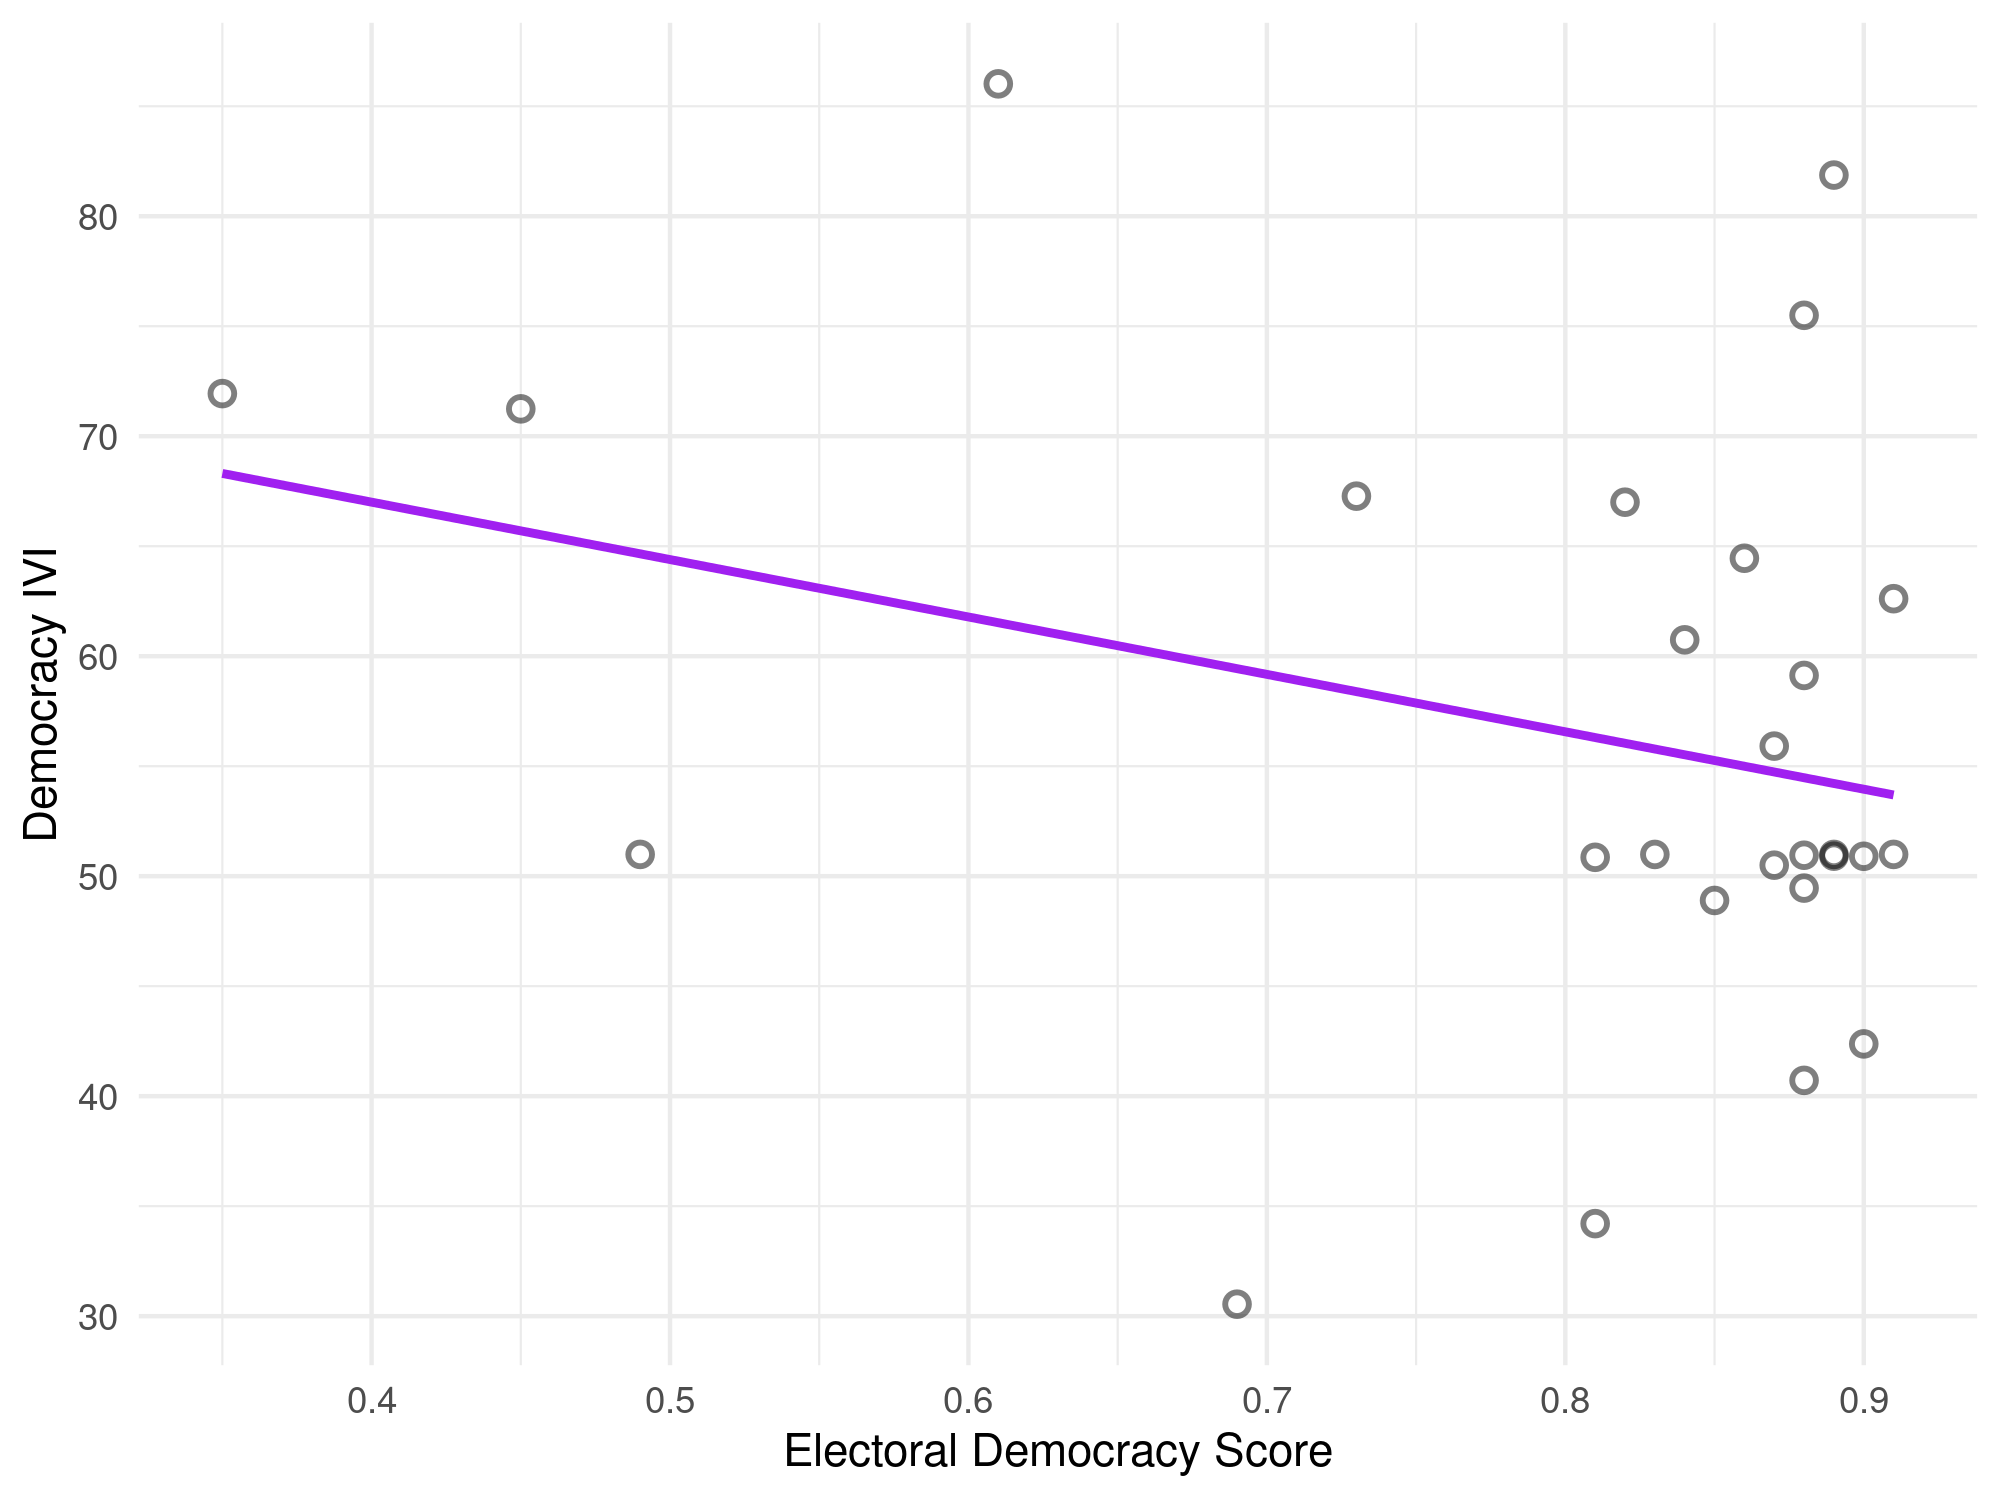
\includegraphics[width=0.75\linewidth]{05-scatter-ED.png}
    \end{minipage}
    \begin{minipage}[c][0.49\textheight][c]{\linewidth}
      \centering
      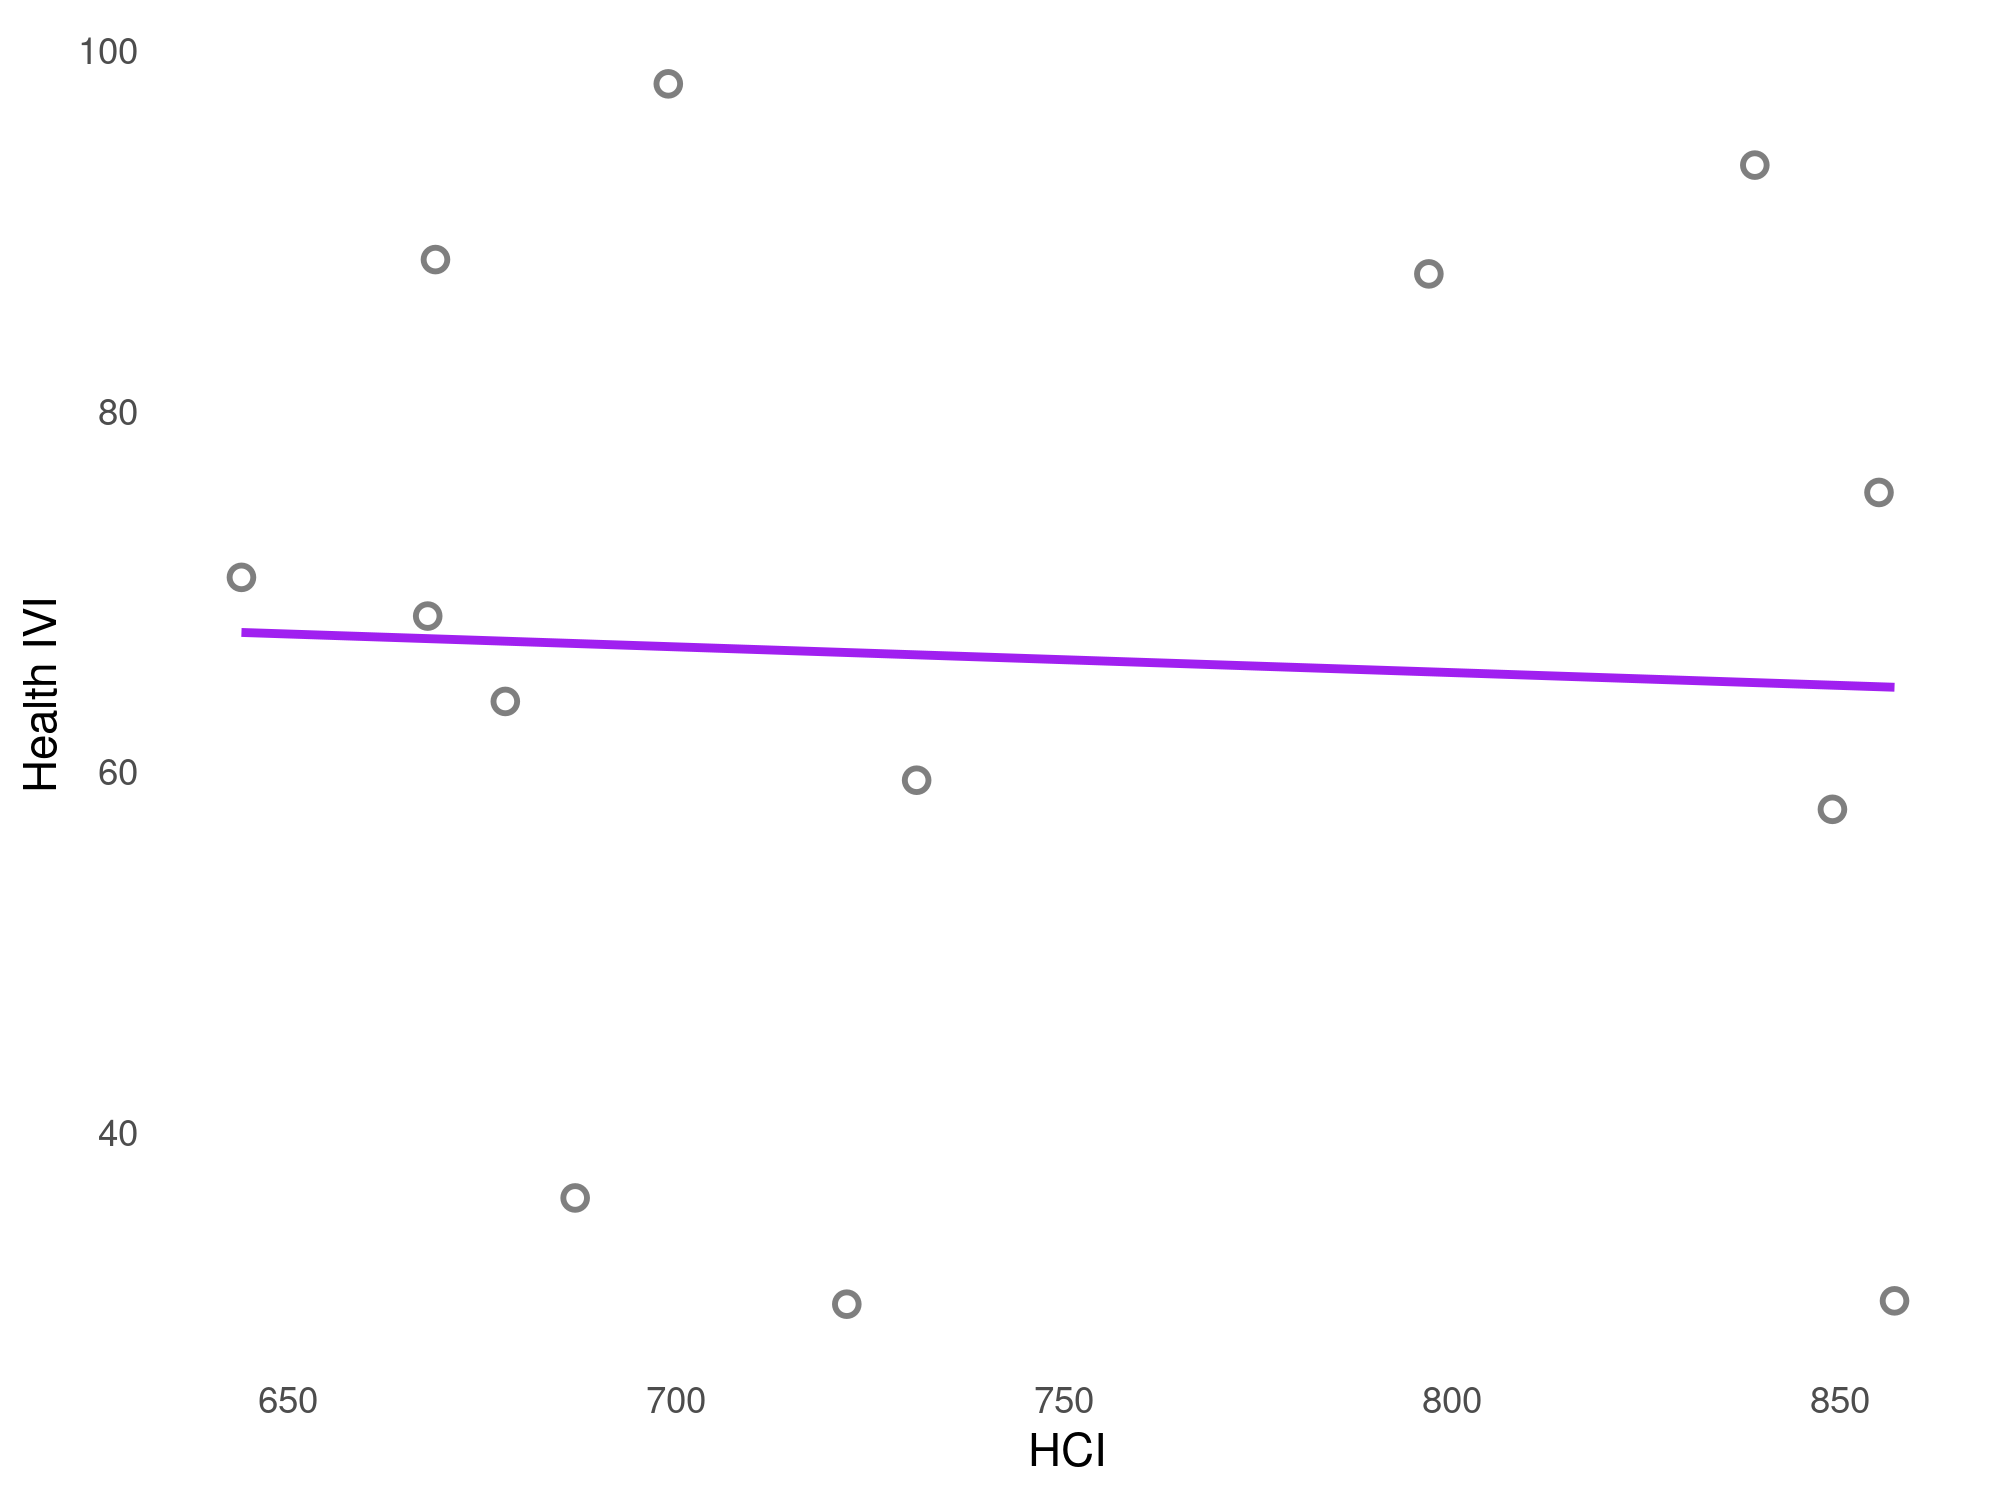
\includegraphics[width=0.75\linewidth]{05-scatter-health.png}
    \end{minipage}
    \column{0.5\textwidth}
    \begin{minipage}[c][0.45\textheight][c]{\linewidth}
      \centering
      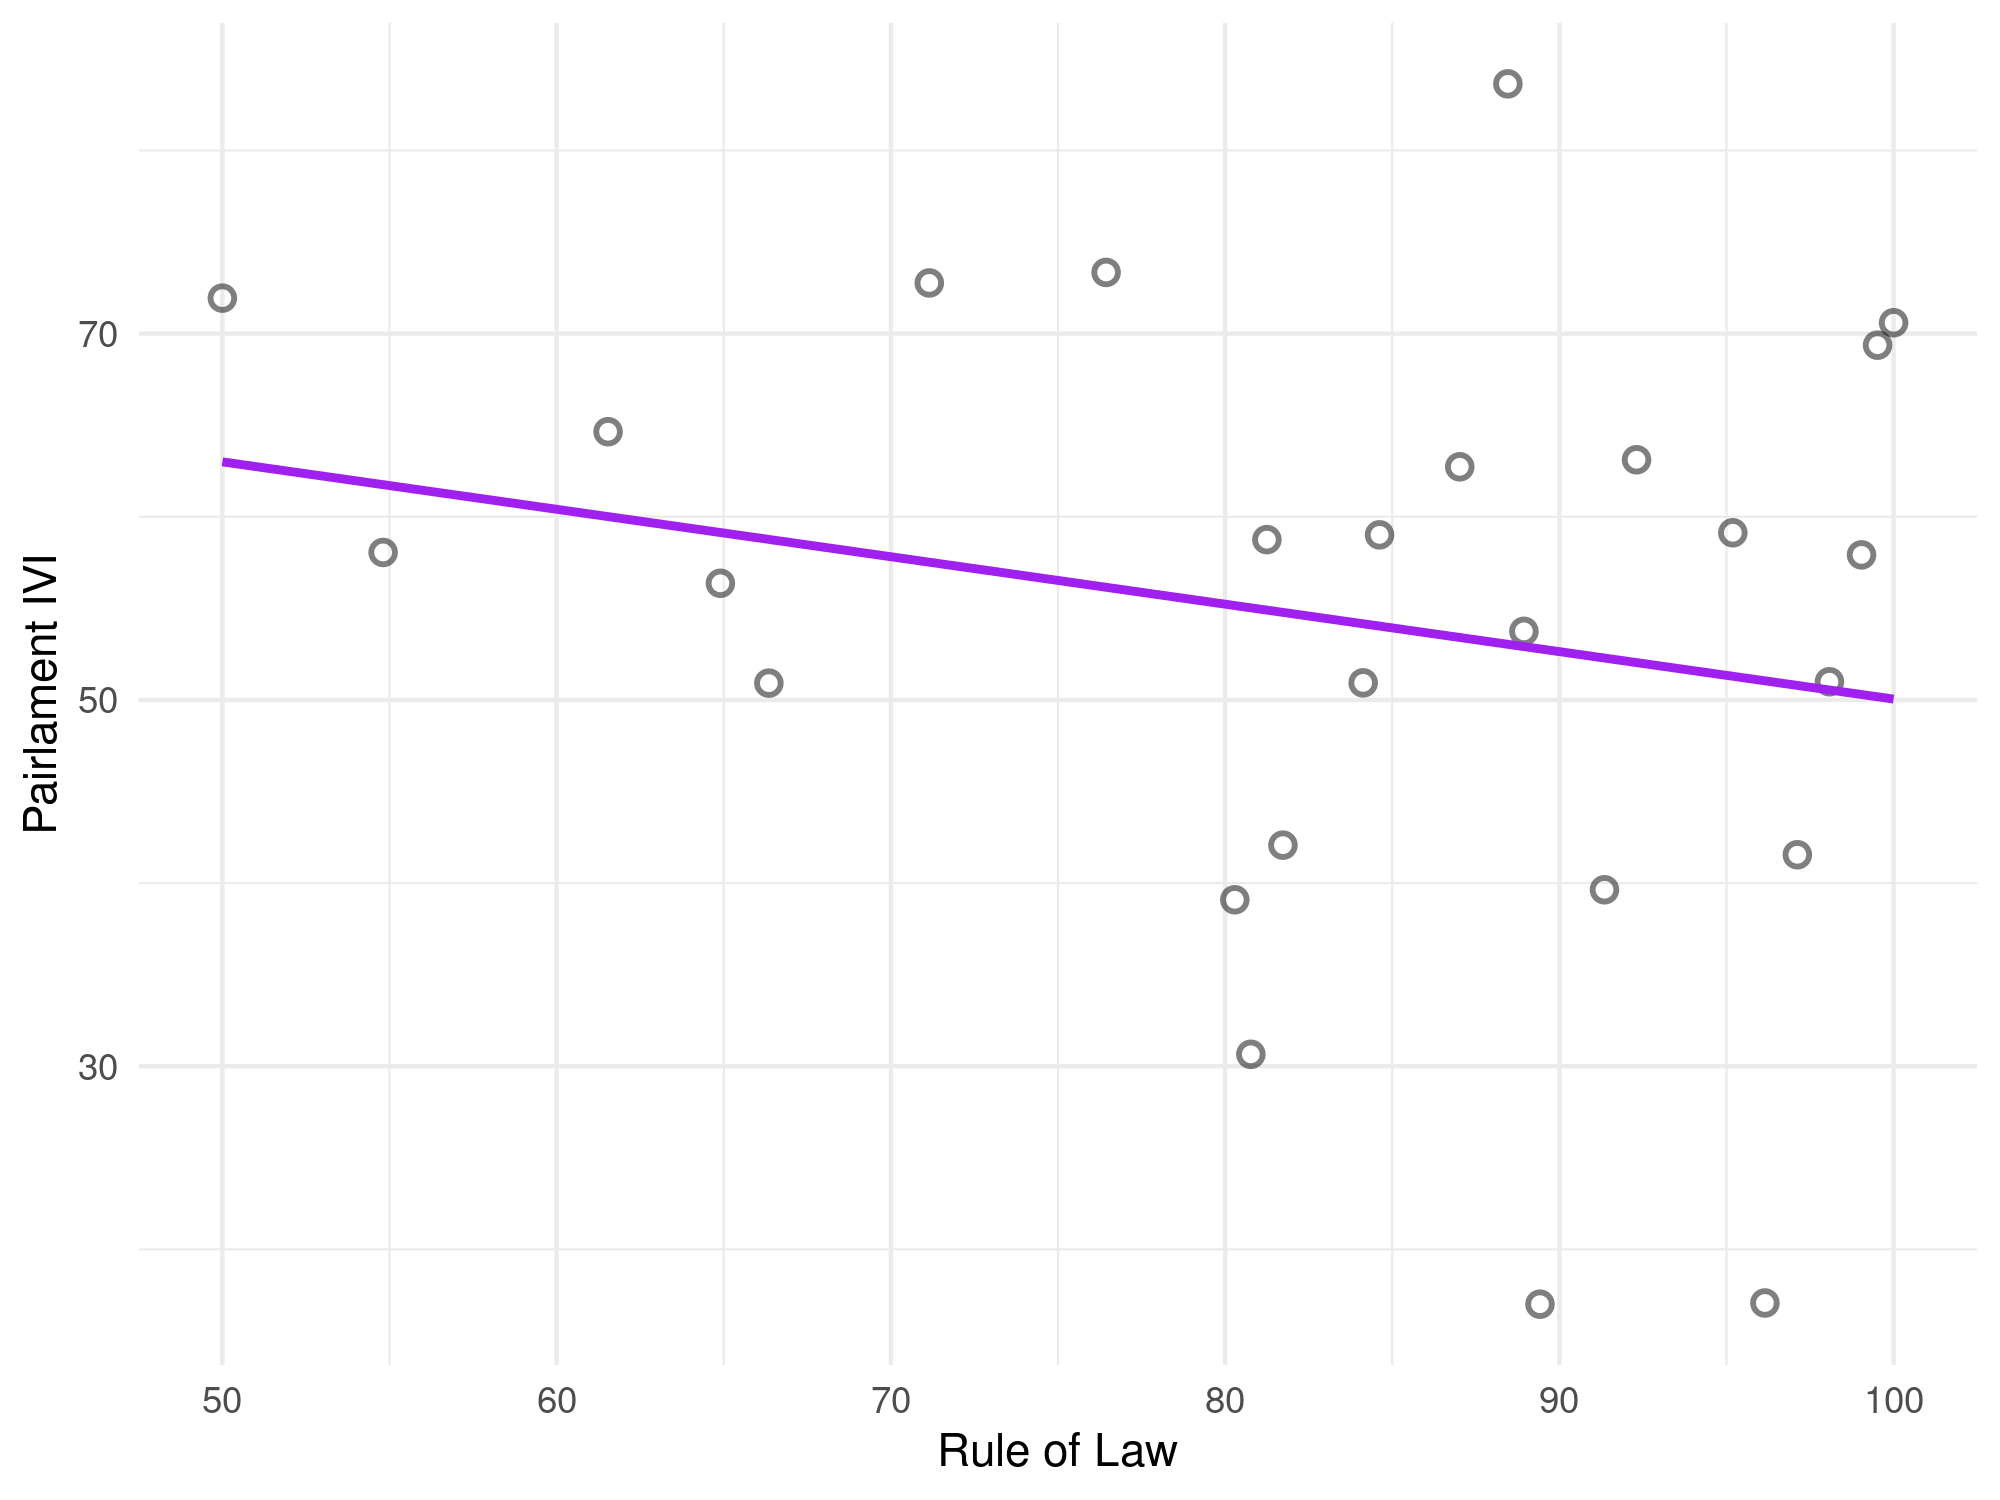
\includegraphics[width=0.75\linewidth]{05-scatter-RoL.png}
    \end{minipage}
  \end{columns}
\end{frame}

\begin{frame}{Summary}

  \begin{itemize}
    \item<+-> After removing redundancies we have fully-connected, simple belief network
    \item<+-> Network structure differences between subgroups (regime type)
    \item<+-> High Influence of beliefs related to problematic domains for a given society
  \end{itemize}

\end{frame}


\begin{frame}{Directions}

  \begin{itemize}
    \item Differences between ruling and opposition parties voters
    \item Pairwise Ising model (binary beliefs)
    \item Compare with other influence/centrality metrics
    \item Investigate time temporal stability in panel surveys
  \end{itemize}
\end{frame}

\begin{frame}

  \begin{center}
    \Large
    \alert{Thank You!} \\
    \vspace{1cm}
    \textbf{github.com/atomashevic/essnet} \\
    \vspace{1cm}
    \alert{atommashevic@ff.uns.ac.rs}
  \end{center}


\end{frame}

\end{document}